

\documentclass[        
    a4paper,          % Tamanho da folha A4
    12pt,             % Tamanho da fonte 12pt
    chapter=TITLE,    % Todos os capitulos devem ter caixa alta
    section=Title,    % Todas as secoes devem ter caixa alta somente na primeira letra
    subsection=Title, % Todas as subsecoes devem ter caixa alta somente na primeira letra
    oneside,          % Usada para impressao em apenas uma face do papel
    english,          % Hifenizacoes em ingles
    spanish,          % Hifenizacoes em espanhol
    brazil,           % Ultimo idioma eh o idioma padrao do documento
    fleqn,            % Comente esta linha se quiser centralizar as equacoes. Comente também a linha 65 abaixo
    hyphens,
    sumario=tradicional,
]{abntex2}

% Remover antes de escrever o TCC


% Importações de pacotes
\usepackage[T1]{fontenc}
\usepackage[utf8]{inputenc}
\usepackage[brazil]{babel}
\usepackage{xcolor}

\usepackage[utf8]{inputenc}                         % Acentuação direta
\usepackage[T1]{fontenc}                            % Codificação da fonte em 8 bits
\usepackage{graphicx}                               % Inserir figuras
\usepackage{amsfonts, amssymb, amsmath}             % Fonte e símbolos matemáticos
\usepackage{booktabs}                               % Comandos para tabelas
\usepackage{verbatim}                               % Texto é interpretado como escrito no documento
\usepackage{multirow, array}                        % Múltiplas linhas e colunas em tabelas
\usepackage{indentfirst}                            % Endenta o primeiro parágrafo de cada seção.
\usepackage{listings}                               % Utilizar codigo fonte no documento
\usepackage{xcolor}
\usepackage{microtype}                              % Para melhorias de justificação?
\usepackage[portuguese,ruled,lined]{algorithm2e}    % Escrever algoritmos
\usepackage{algorithmic}                            % Criar Algoritmos  
%\usepackage{float}                                 % Utilizado para criação de floats
\usepackage{amsgen}
\usepackage{lipsum}                                 % Usar a simulação de texto Lorem Ipsum
%\usepackage{titlesec}                              % Permite alterar os títulos do documento
\usepackage{tocloft}         % Permite alterar a formatação do Sumário
\usepackage{etoolbox}                               % Usado para alterar a fonte da Section no Sumário
\usepackage[nogroupskip,nonumberlist]{glossaries}   % Permite fazer o glossario

\usepackage[font={singlespacing},format=plain,skip=0pt,singlelinecheck = false]{caption}            % Altera o comportamento da tag caption

\usepackage[alf, abnt-emphasize=bf, recuo=0cm, abnt-etal-cite=3, abnt-etal-list=0, abnt-etal-text=it, bibjustif]{abntex2cite}  % Citações padrão ABNT
%\usepackage[bottom]{footmisc}                      % Mantém as notas de rodapé sempre na mesma posição
%\usepackage{times}                                 % Usa a fonte Times
%%%%%%%%%%%%%%%%%%% AVISO %%%%%%%%%%%%%%%%%%%%%%%%%%%%%%%%%%%%%%%%
%descomente as duas linhas abaixo para alterar o texto de Times New Roman para Arial:

%\usepackage{helvet}
%\renewcommand{\familydefault}{\sfdefault}  % Usa a fonte Arial              
%%%%%%%%%%%%%%%%%%%%%%%%%%%%%%%%%%%%%%%%%%%%%%%%%%%%%%%%%%%%%%%%%%

\usepackage{mathptmx}         % Usa a fonte Times New Roman			%\usepackage{lmodern}         % Usa a fonte Latin Modern
%\usepackage{subfig}          % Posicionamento de figuras
%\usepackage{scalefnt}        % Permite redimensionar tamanho da fonte
%\usepackage{color, colortbl} % Comandos de cores
%\usepackage{lscape}          % Permite páginas em modo "paisagem"
%\usepackage{ae, aecompl}     % Fontes de alta qualidade
%\usepackage{picinpar}        % Dispor imagens em parágrafos
%\usepackage{latexsym}        % Símbolos matemáticos
%\usepackage{upgreek}         % Fonte letras gregas
\usepackage{appendix}         % Gerar o apendice no final do documento
\usepackage{paracol}          % Criar paragrafos sem identacao
\usepackage{lib/ufersatex}	      % Biblioteca com as normas para trabalhos academicos
\usepackage{pdfpages}         % Incluir pdf no documento
\usepackage{amsmath}          % Usar equacoes matematicas

% importar meus pacotes
\usepackage{setspace}

\makeglossaries % Organiza e gera a lista de abreviaturas, simbolos e glossario
% use o comando \gls{} ao citar no texto para a sigla ficar visível na Lista. Caso a lista de abreviaturas não estiver aparecendo é porque você não utilizou o comando "gls" no texto. Exemplo no texto:   De acordo com o \gls{MCEG} ...  
\newacronym{PDF}{PDF}{\textit{Portable Document Format}}
\newacronym{API}{API}{\textit{Application Programming Interface}}
\newacronym{DQN}{DQN}{\textit{Deep Q-Network}}
\newacronym{EV}{EV}{\textit{Expected Value}}
\newacronym{GPU}{GPU}{\textit{Graphics Processing Unit}}
\newacronym{HTML}{HTML}{\textit{HyperText Markup Language}}
\newacronym{HTTP}{HTTP}{\textit{Hypertext Transfer Protocol}}
\newacronym{IA}{IA}{Inteligência Artificial}
\newacronym{JSON}{JSON}{\textit{JavaScript Object Notation}}
\newacronym{MCCFR}{MCCFR}{\textit{Monte Carlo Counterfactual Regret Minimization}}
\newacronym{MCTS}{MCTS}{\textit{Monte Carlo Tree Search}}
\newacronym{MVC}{MVC}{\textit{Model-View-Controller}}
\newacronym{PARC}{PARC}{\textit{Palo Alto Research Center}}
\newacronym{ReLU}{ReLU}{\textit{Rectified Linear Unit}}
\newacronym{RNA}{RNA}{Rede Neural Artificial}
\newacronym{SIGAA}{SIGAA}{Sistema Integrado de Gestão de Atividades Acadêmicas}
\newacronym{SISBI}{SISBI}{Sistema de Bibliotecas da UFERSA}
\newacronym{SUTIC}{SUTIC}{Superintendência de Tecnologia da Informação e Comunicação}
\newacronym{TCC}{TCC}{Trabalho de Conclusão de Curso}
\newacronym{UFERSA}{UFERSA}{Universidade Federal Rural do Semi-Árido}
\newacronym{USP}{USP}{Universidade de São Paulo} % Carrega as definições de siglas e abreviaturas
\makeindex      % Gera o Indice do documento

\usepackage{chngcntr}
\counterwithout*{footnote}{chapter}

\usepackage{listings}
\usepackage{xcolor} % Opcional, para melhorar as cores

% Configuração básica para o código não vazar da página e ter números nas linhas
\lstset{
    basicstyle=\ttfamily\footnotesize,
    breaklines=true,
    frame=single,
    numbers=left,
    numberstyle=\tiny\color{gray}
}

\usepackage{color}

% Cartas de pôquer em estilo simples e estável para uso inline
\newcommand{\pokercard}[3]{%
    {\setlength{\fboxsep}{0.35ex}%
        \textcolor{#2}{\fbox{\sffamily\bfseries #1\ensuremath{#3}}}%
    }%
}
\newcommand{\As}{\pokercard{A}{black}{\spadesuit}}
\newcommand{\Ah}{\pokercard{A}{red}{\heartsuit}}
\newcommand{\Ad}{\pokercard{A}{red}{\diamondsuit}}
\newcommand{\Ac}{\pokercard{A}{black}{\clubsuit}}
\newcommand{\Ks}{\pokercard{K}{black}{\spadesuit}}
\newcommand{\Kh}{\pokercard{K}{red}{\heartsuit}}
\newcommand{\Kd}{\pokercard{K}{red}{\diamondsuit}}
\newcommand{\Kc}{\pokercard{K}{black}{\clubsuit}}
\newcommand{\Qs}{\pokercard{Q}{black}{\spadesuit}}
\newcommand{\Qh}{\pokercard{Q}{red}{\heartsuit}}
\newcommand{\Qd}{\pokercard{Q}{red}{\diamondsuit}}
\newcommand{\Qc}{\pokercard{Q}{black}{\clubsuit}}
\newcommand{\Js}{\pokercard{J}{black}{\spadesuit}}
\newcommand{\Jh}{\pokercard{J}{red}{\heartsuit}}
\newcommand{\Jd}{\pokercard{J}{red}{\diamondsuit}}
\newcommand{\Jc}{\pokercard{J}{black}{\clubsuit}}
\newcommand{\tens}{\pokercard{10}{black}{\spadesuit}}
\newcommand{\tenh}{\pokercard{10}{red}{\heartsuit}}
\newcommand{\tend}{\pokercard{10}{red}{\diamondsuit}}
\newcommand{\tenc}{\pokercard{10}{black}{\clubsuit}}
\newcommand{\nines}{\pokercard{9}{black}{\spadesuit}}
\newcommand{\nineh}{\pokercard{9}{red}{\heartsuit}}
\newcommand{\nined}{\pokercard{9}{red}{\diamondsuit}}
\newcommand{\ninec}{\pokercard{9}{black}{\clubsuit}}
\newcommand{\eigs}{\pokercard{8}{black}{\spadesuit}}
\newcommand{\eigh}{\pokercard{8}{red}{\heartsuit}}
\newcommand{\eigd}{\pokercard{8}{red}{\diamondsuit}}
\newcommand{\eigc}{\pokercard{8}{black}{\clubsuit}}
\newcommand{\sevs}{\pokercard{7}{black}{\spadesuit}}
\newcommand{\sevh}{\pokercard{7}{red}{\heartsuit}}
\newcommand{\sevd}{\pokercard{7}{red}{\diamondsuit}}
\newcommand{\sevc}{\pokercard{7}{black}{\clubsuit}}
\newcommand{\sixs}{\pokercard{6}{black}{\spadesuit}}
\newcommand{\sixh}{\pokercard{6}{red}{\heartsuit}}
\newcommand{\sixd}{\pokercard{6}{red}{\diamondsuit}}
\newcommand{\sixc}{\pokercard{6}{black}{\clubsuit}}
\newcommand{\fives}{\pokercard{5}{black}{\spadesuit}}
\newcommand{\fiveh}{\pokercard{5}{red}{\heartsuit}}
\newcommand{\fived}{\pokercard{5}{red}{\diamondsuit}}
\newcommand{\fivec}{\pokercard{5}{black}{\clubsuit}}
\newcommand{\fours}{\pokercard{4}{black}{\spadesuit}}
\newcommand{\fourh}{\pokercard{4}{red}{\heartsuit}}
\newcommand{\fourd}{\pokercard{4}{red}{\diamondsuit}}
\newcommand{\fourc}{\pokercard{4}{black}{\clubsuit}}
\newcommand{\tres}{\pokercard{3}{black}{\spadesuit}}
\newcommand{\treh}{\pokercard{3}{red}{\heartsuit}}
\newcommand{\tred}{\pokercard{3}{red}{\diamondsuit}}
\newcommand{\trec}{\pokercard{3}{black}{\clubsuit}}
\newcommand{\twos}{\pokercard{2}{black}{\spadesuit}}
\newcommand{\twoh}{\pokercard{2}{red}{\heartsuit}}
\newcommand{\twod}{\pokercard{2}{red}{\diamondsuit}}
\newcommand{\twoc}{\pokercard{2}{black}{\clubsuit}}

% Definindo algumas cores bonitas para o código
\definecolor{lightgray}{rgb}{0.95, 0.95, 0.95}
\definecolor{darkgray}{rgb}{0.4, 0.4, 0.4}
\definecolor{purple}{rgb}{0.65, 0.12, 0.82}
\definecolor{blue}{rgb}{0.13, 0.13, 1}
\definecolor{green}{rgb}{0, 0.5, 0}

% Criando a definição do JavaScript
\lstdefinelanguage{JavaScript}{
    keywords={typeof, new, true, false, catch, function, return, null, catch, switch, var, let, const, if, in, while, do, else, case, break},
    keywordstyle=\color{blue}\bfseries,
    ndkeywords={class, export, boolean, throw, implements, import, this},
    ndkeywordstyle=\color{darkgray}\bfseries,
    identifierstyle=\color{black},
    sensitive=false,
    comment=[l]{//},
    morecomment=[s]{/*}{*/},
    commentstyle=\color{green}\ttfamily,
    stringstyle=\color{purple}\ttfamily,
    morestring=[b]',
    morestring=[b]"
}

% Configurando o padrão do listings para usar o que acabamos de criar
\lstset{
    language=JavaScript,
    backgroundcolor=\color{lightgray},
    extendedchars=true,
    basicstyle=\footnotesize\ttfamily,
    showstringspaces=false,
    showspaces=false,
    numbers=left,
    numberstyle=\tiny\color{gray},
    numbersep=9pt,
    tabsize=2,
    breaklines=true,
    showtabs=false,
    captionpos=b
}

\lstset{
    basicstyle=\ttfamily\footnotesize,
    breaklines=true,
    frame=single,
    showstringspaces=false,
    numbers=none,
    backgroundcolor=\color{gray!10},
    % --- SOLUÇÃO DOS ACENTOS AQUI ---
    literate=
        {á}{{\'a}}1 {é}{{\'e}}1 {í}{{\'i}}1 {ó}{{\'o}}1 {ú}{{\'u}}1
        {Á}{{\'A}}1 {É}{{\'E}}1 {Í}{{\'I}}1 {Ó}{{\'O}}1 {Ú}{{\'U}}1
        {à}{{\`a}}1 {è}{{\`e}}1 {ì}{{\`i}}1 {ò}{{\`o}}1 {ù}{{\`u}}1
        {À}{{\`A}}1 {È}{{\'E}}1 {Ì}{{\`I}}1 {Ò}{{\`O}}1 {Ù}{{\`U}}1
        {â}{{\^a}}1 {ê}{{\^e}}1 {î}{{\^i}}1 {ô}{{\^o}}1 {û}{{\^u}}1
        {Â}{{\^A}}1 {Ê}{{\^E}}1 {Î}{{\^I}}1 {Ô}{{\^O}}1 {Û}{{\^U}}1
        {ã}{{\~a}}1 {õ}{{\~o}}1 {Ã}{{\~A}}1 {Õ}{{\~O}}1
        {ç}{{\c c}}1 {Ç}{{\c C}}1
}

\setlength{\mathindent}{0pt} %Complementa o alinhamento de equações para totalmente a esquerda.

%%%%%%%%%%%%%%%%%%%%%%%%%%%%%%%%%%%%%%%%%%%%%%%%%%%%%
%%                     ATENCAO                     %%
%%%%%%%%%%%%%%%%%%%%%%%%%%%%%%%%%%%%%%%%%%%%%%%%%%%%%
%  Qual e o nivel do trabalho academico que voce esta 
% escrevendo? Retire o simbolo "%" apenas de um dos 
% quatro topicos abaixo refente ao nível do seu traba
% -lho.

\trabalhoacademico{tccgraduacao}

%%%%%%%%%%%%%%%%%%%%%%%%%%%%%%%%%%%%%%%%%%%%%%%%%%%%%
% Remove as bordas vermelhas e verdes do PDF gerado
% Coloque 'sim' pare remover

\removerbordasdohyperlink{sim} 

% Adiciona a cor Azul a todos os hyperlinks

\cordohyperlink{nao}

%%%%%%%%%%%%%%%%%%%%%%%%%%%%%%%%%%%%%%%%%%%%%%%%%%%%%
%%         Informacao sobre a instituicao          %%
%%%%%%%%%%%%%%%%%%%%%%%%%%%%%%%%%%%%%%%%%%%%%%%%%%%%%

\ies{Universidade Federal Rural do Semi-Árido}
\iessigla{UFERSA}
\centro{Pró-Reitoria de Graduação}
\departamento{Departamento de Engenharias e Tecnologia}

%%%%%%%%%%%%%%%%%%%%%%%%%%%%%%%%%%%%%%%%%%%%%%%%%%%%%
%%        Informacao para TCC de Graduacao         %%
%%%%%%%%%%%%%%%%%%%%%%%%%%%%%%%%%%%%%%%%%%%%%%%%%%%%%

\graduacaoem{INTERDISCIPLINAR EM TECNOLOGIA DA INFORMAÇÃO/CMPF}
\habilitacao{bacharel} % Ou licenciado(a)

% AVISO: Caso necessario alterar o texto de apresenta-
% cao da Especializacao, ir a pasta "lib", arquivo 
% "ppgcctex.sty" na linha 502.

%%%%%%%%%%%%%%%%%%%%%%%%%%%%%%%%%%%%%%%%%%%%%%%%%%%%%
%%      Informacoes relacionadas ao trabalho       %%
%%%%%%%%%%%%%%%%%%%%%%%%%%%%%%%%%%%%%%%%%%%%%%%%%%%%%

\autor{Pedro Hércules Souza Grangeiro} 
\titulo{Inteligência Artificial Aplicada ao Texas Hold'em: Uma Abordagem com Aprendizado por Reforço Profundo e Algoritmo de Predição Monte Carlo}
\data{2026}
\local{Pau dos Ferros}

% Exemplo: \dataaprovacao{01 de Janeiro de 2023}
\dataaprovacao{\underline{  }}

%%%%%%%%%%%%%%%%%%%%%%%%%%%%%%%%%%%%%%%%%%%%%%%%%%%%%
%%           Informação sobre o Orientador         %%
%%%%%%%%%%%%%%%%%%%%%%%%%%%%%%%%%%%%%%%%%%%%%%%%%%%%%

\orientador{Kennedy Reurison Lopes}
\titulacaoOrientador{Prof. Dr.}
\orientadories{UFERSA}
\orientadorcentro{} % opicional
\orientadorfeminino{nao} % Coloque 'sim' se for do sexo feminino

%%%%%%%%%%%%%%%%%%%%%%%%%%%%%%%%%%%%%%%%%%%%%%%%%%%%%
%%          Informação sobre o Coorientador        %%
%%%%%%%%%%%%%%%%%%%%%%%%%%%%%%%%%%%%%%%%%%%%%%%%%%%%%

% Deixe o nome do coorientador em branco para remover do documento

\coorientador{}
\coorientadories{SIGLA}
\coorientadorcentro{Centro do Coorientador (SIGLA)} % opicional
\coorientadorfeminino{nao} % Coloque 'sim' se for do sexo feminino

%%%%%%%%%%%%%%%%%%%%%%%%%%%%%%%%%%%%%%%%%%%%%%%%%%%%%
%%              Informação sobre a banca           %%
%%%%%%%%%%%%%%%%%%%%%%%%%%%%%%%%%%%%%%%%%%%%%%%%%%%%%

% Atenção! Deixe em branco o nome do membro da banca para remover da folha de aprovacao

% Exemplo de uso:
% \membrodabancadois{Prof. Dr. Fulano de Tal}
% \membrodabancadoisies{Universidade Federal do Ceará - UFC}

\membrodabancadois{Rosana Cibely Batista Rego}
\titulacaoBancaDois{Profa. Dra.}
\membrodabancadoiscentro{}
\membrodabancadoisies{UFERSA}
\membrodabancatres{Marcos Daniel Nogueira Maia}
\titulacaoBancaTres{Prof. Dr.}
\membrodabancatrescentro{}
\membrodabancatresies{UFERSA}
\membrodabancaquatro{}
\membrodabancaquatrocentro{}
\membrodabancaquatroies{SIGLA}
\membrodabancacinco{Prof. Dr. Xxxxxxx Xxxxxx Xxxxxxx}
\membrodabancacincocentro{Teste}
\membrodabancacincoies{Universidade do Membro da Banca Cinco (SIGLA)}
\membrodabancaseis{Prof. Dr. Xxxxxxx Xxxxxx Xxxxxxx}
\membrodabancaseiscentro{}
\membrodabancaseisies{Universidade do Membro da Banca Seis (SIGLA)}

% Para espacaomento duplo nas referencias
% \let\OLDthebibliography\thebibliography
% \renewcommand\thebibliography[1]{
% \OLDthebibliography{#1}
% \setlength{\itemsep}{24pt} % Space between items
% \setlength{\parskip}{0pt} % Space between paragraphs
% }

\begin{document}

% Elementos pré-textuais
\imprimircapa
\imprimirfolhaderosto{}
\imprimirfichacatalografica{1-pre-textuais/ficha-catalografica} %  gerada pela biblioteca 
\imprimirfolhadeaprovacao
\imprimirdedicatoria{1-pre-textuais/dedicatoria}
\imprimiragradecimentos{1-pre-textuais/agradecimentos}
\imprimirepigrafe{1-pre-textuais/epigrafe}
\imprimirresumo{1-pre-textuais/resumo}
\imprimirabstract{1-pre-textuais/abstract}
\glsaddallunused
\renewcommand*\listfigurename{Lista de Figuras} %Se você comentar esta linha o título da lista fica: LISTA DE ILUSTRAÇÕES
\imprimirlistadeilustracoes
% \imprimirlistadetabelas
%\imprimirlistadequadros
%\imprimirlistadealgoritmos
%\imprimirlistadecodigosfonte
\imprimirlistadeabreviaturasesiglas
\imprimirlistadesimbolos{1-pre-textuais/lista-de-simbolos}
\imprimirsumario

\setcounter{table}{0}% Deixe este comando antes da primeira tabela.

%Elementos textuais
\textual
\chapter{Introdução}
\label{cap:introducao}

O poquêr, particularmente a modalidade \textit{Texas Hold'Em}, é considerado um dos maiores desafios atuais para a inteligência artificial, pois envolve aspectos vitais como a tomada de decisão diante da incerteza, gerenciamento de risco e a necessidade de entender o comportamento dos oponentes. Ao contrário de jogos tradicionais como xadrez e \textit{Go}, onde todas as informações estão disponíveis para os jogadores, o poquêr apresenta a característica de informação incompleta, exigindo decisões baseadas em dados parciais e sob a influência de elementos aleatórios. Essa particularidade tem incentivado o desenvolvimento de novas técnicas em \textit{machine learning}, com foco especial em aprendizado de máquina e modelagem probabilística.

Neste cenário, os métodos que utilizam redes neurais artificiais têm se tornado cada vez mais significativos, sendo capazes de identificar padrões complexos a partir de extensas quantidades de dados, sem depender diretamente do conhecimento anterior do programador. O processo de treinamento desses modelos, que pode ser supervisionado, não supervisionado ou por reforço, possibilita a identificação de táticas de jogo, a previsão de jogadas dos adversários e a realização de escolhas otimizadas, fundamentais na mecânica do poquêr.

Contudo, a complexidade do espaço de estados no \textit{Texas Hold'Em}, devido ao enorme número de combinações possíveis de cartas, apostas e estilos de jogo dos oponentes, torna impraticável a exploração de todas as opções disponíveis através de métodos convencionais. Para contornar esse desafio, destacam-se os algoritmos de \textit{Monte Carlo}, incluindo o \gls{MCTS} e o \gls{MCCFR}, que conseguem analisar amostras selecionadas das possibilidades do jogo, estimando chances de ganhar, retorno esperado e ajustando estratégias em tempo real. Essa metodologia simula diversos cenários possíveis, utilizando redes neurais para determinar os melhores caminhos, mesmo com limitações computacionais.

As mais recentes inovações neste campo envolvem a combinação de métodos de \textit{Monte Carlo} com arquiteturas de redes neurais profundas, como as redes \textit{actor-critic}, permitindo que o agente se desenvolva através de autojogo e levando a políticas que se aproximam do equilíbrio de Nash, um padrão de referência em jogos de soma zero. Exemplos como \textit{DeepStack}, \textit{Libratus} e \textit{Pluribus} evidenciam a eficácia dessas ferramentas ao vencer campeões mundiais em competições reais, revelando táticas sólidas para partidas entre dois jogadores e também em ambientes com múltiplos competidores.

Dessa forma, a criação de uma rede neural capaz de jogar poquêr \textit{Texas Hold’Em} utilizando técnicas de \textit{Monte Carlo} fornece uma contribuição significativa para o entendimento da IA aplicada a decisões complexas. Este estudo tem como objetivo executar modelagem teórica até práticas em ambientes simulados, demonstrando como a união entre aprendizado profundo e simulações probabilísticas pode resultar em agentes de alto desempenho em cenários com informações incompletas e vários adversários.

\chapter{Fundamentação teórica}
\label{cap:fundamentacao-teorica}
\section{O jogo pôquer Texas Hold'Em}

O pôquer é um dos jogos mais populares da história, como dito por como falado por \citeonline{barbosa2005confiabilidade}, possuindo várias modalidades, sendo algumas como o pôquer \textit{Head's Up}, que consiste em um contra um direto, sendo a modalidade mais famosa a \textit{Texas Hold'Em}, o pôquer é um jogo composto por muitos fatores, sendo os mais importantes para entende-lo os seguintes:

\subsection{A hierarquia das cartas}

Diferentemente dos jogos que envolvem o baralho, no pôquer, o ás é a carta de maior valor, sendo a seguinte hierarquia das cartas:

\begin{enumerate}
      \item Dois(2) \twos
      \item Três(3) \tres
      \item Quatro(4) \fours
      \item Cinco(5) \fives
      \item Seis(6) \sixs
      \item Sete(7) \sevs
      \item Oito(8) \eigs
      \item Nove(9) \nines
      \item Dez(10) \tens
      \item Valete(J) \Js
      \item Dama(Q) \Qs
      \item Rei(K) \Ks
      \item Ás (A) \As
\end{enumerate}

sendo essa a ordem crescente dos valores das cartas do pôquer, é importante destacar que o naipe não influencia no fator de valor das cartas, sendo assim, um 8 de espadas e um 8 de paus têm o mesmo valor.

\subsection{A configuração da modalidade}

No \textit{Texas Hold'Em} cada jogador recebe duas cartas aleatórias do baralho, que é o que chamado de ``mão'', sendo essas cartas que apenas o jogador tem acesso, enquanto isso, são distribuidas ao decorrer do jogo mais cinco cartas de forma comunitárias, as cartas comunitárias são cartas que todos os jogadores tem acesso e podem formar o jogos do pôquer.

\subsection{As combinações e o desempate}

O principal objetivo do pôquer é formar combinações de cinco cartas, sendo um conjunto formado pelas duas cartas da mão do jogador com as cinco cartas comunitárias, sempre descartando as duas cartas de menor valor.

As combinações do pôquer são as seguintes em ordem decrescente de força, sendo a primeira a mais forte e a última a mais fraca:

\begin{itemize}
      \item \textit{Straight Flush}:
            É a maior combinação do pôquer, que consiste em cinco cartas em sequência, sendo todas elas do mesmo naipe, sendo em caso de empate, se sobressai o jogador que tiver a maior sequencia, que pode ser dita como a que termina com a carta de maior valor, dentro dela se encontra o maior jogo possível do pôquer, que é o \textit{Royal Straight Flush} que consiste na sequencia das maiores cartas, do dez até o ás, do mesmo naipe, que é a mostrada no exemplo abaixo:

            $$ \tenc \Jc \Qc \Kc \Ac $$
      \item \textit{Quadra}:
            A quadra são quatro cartas de mesmo valor, o desempate é feito pela maior quadra,da seguinte forma:

            $$ \Ac \Ad \As \Ah \sevc$$
      \item \textit{Full House}:
            Consiste no jogador formar uma combinação com uma trinca e um par, o desempate é feito pela maior trica, caso as trincas sejam iguais, é dada pelo maior par, podendo ser visto da seguinte forma:

            $$ \Ac \Ah \As \Kc \Kh$$
      \item \textit{Flush}:
            Ocorre quando as cinco cartas da combinação do jogador tem o mesmo naipe, o desempate é feito pela maior carta de cada jogador, caso seja a mesma, a seguinte maior carta do jogador é o desempate, assim sucessivamente até a quinta carta caso seja necessário, um \textit{flush} pode ser visto como:

            $$ \Ah \Kh \Qh \nineh \twoh$$

      \item \textit{Straight}:
            É a sequência de cinco cartas sem importar o naipe das cartas que a compõem, o desempate é feito pela maior sequencia, segue um exemplo de \textit{straight}:

            $$ \Ac \twoh \tres \fourd \fivec$$
      \item Trinca:
            É uma combinação formada por três cartas de mesmo valor, o desempate é feito pela maior trinca, a trinca pode ser vista como:

            $$ \trec \tred \treh \Ac \twoh$$
      \item Dois pares:
            Consiste no jogador formar dois pares de cartas do mesmo valor, sem importar o naipe, sendo o desempate feito pelo maior par dentre os dois pares, caso o primeiro maior par seja igual entre os jogadores, o segundo par é o quesito de desempate, um exemplo de dois pares é:

            $$ \Ac \Ah \twoc \twoh \tres$$
      \item Par:
            É quando o jogador forma um par de duas cartas de mesmo valor, sem importar o naipe, o desempate é feito pelo maior par, segue um exemplo de par:

            $$ \Qc \Qh \twoc \fourd \sevh$$
      \item Carta alta:
            Caso nenhum dos jogadores tenha formado nenhuma combinação, o vencedor é aquele que tiver a maior carta em sua mão, o desempate é feito comparando a maior carta dos jogadores, se for a mesma, a próxima verificada é a segunda maior, assim por diante até a quinta carta de cada um, segue um exemplo de jogo de carta alta:

            $$ \Ac \twoc \fourd \sevs \Kh$$
\end{itemize}

É válido elucidar que as sequencias no pôquer tem um limite, sempre começando no ás, quando se segue do ás até o cinco, sendo a menor sequencia possível, e sempre terminam no ás, sendo a maior sequencia possivel a que vai do dez até o ás, sendo assim as sequencias não são um ciclo, são uma linha fechada.

\subsection{O desempate}
Já foi citado o desempate especifico de cada combinação acima, entretanto, em raros casos, quando dois jogadores possuem a mesma combinação, é necessário aplicar outro metodo de desempate, que é conhecido como \textit{kicker}, considerando o seguinte cenário de empate entre dois jogadores:

Jogador 1 possui: \fivec \fived \twoc \twod \Ah

Jogador 2 possui: \fiveh \fives \twoh \twos \fourd

Nesse caso os dois jogadores possuem dois pares de mesmos valores, sendo assim, o \textit{kicker} é a maior carta fora da combinação, nesse caso sendo o ás para o jogador 1 e o quatro para o jogador 2, sendo assim, o jogador 1 possui o \textit{kicker} maior, dando a ele a vitória.

\subsection{As fases de aposta}

No pôquer, as apostas seguem o sentido horário dos jogadores, sempre se mantendo nesse sentido.
O \textit{Texas hold'Em} possui cinco fases de aposta, que são os momentos que os jogadores podem apostar suas fichas, sendo elas:

\begin{itemize}
      \item \textit{Pre-Flop}

            É quando os jogadores recebem suas duas cartas privadas, sem saber quais as cartas de seus adversários, nessa fase não existem cartas comunitárias, além de ser a única fase de apostas obrigatórias, em que o jogador precisa apostar se desejar participar da rodada.

      \item \textit{Flop}

            São viradas três cartas comunitárias, ocorrendo mais uma rodada de apostas opcionais, que caso um dos jogadores aposte, todos os outros que quiserem se manter na rodada devem apostar tambem.

      \item \textit{River}

            É virada a quarta carta comunitária, seguindo a mesma lógica de apostas do \textit{flop}.

      \item \textit{Turn}:

            É virada a última carta comunitária, seguindo a mesma lógica de apostas das duas fases anteriores, após o \textit{turn} é executado o \textit{showdown}, que consiste nos jogadores remanescentes da rodada mostrarem sua mão para definir o vencedor.
\end{itemize}

\subsection{As ações do jogador}

Dentro de cada fase de apostas, o jogador pode tomar cinco ações, sempre respeitando seu momento de tomar ações,sendo elas:

\begin{itemize}
      \item \textit{Bet}:
            É quando o jogador aposta uma quantia de fichas;

      \item \textit{Call}:
            Consiste em o jogador pagar uma aposta que outro jogador fez;

      \item \textit{Check}:
            Quando o jogador não quer apostar, ou quando não há apostas para serem cobridas, o jogador pode dar \textit{check}, que funciona como uma passada de vez sem penalidades;

      \item \textit{Raise}:
            O jogador pode dar um \textit{raise} quando quer aumentar uma aposta que outro jogador fez, sendo que um \textit{raise} deve sempre ser o no minimo o dobro da aposta que o mesmo quer aumentar;

      \item \textit{Fold}:
            Consiste na desistencia do jogador, o mesmo desiste da mão e entrega as cartas, perdendo o valor que apostou anteriormente caso tenha apostado;

      \item \textit{All-in}:
            É quando o jogador aposta todas as suas fichas disponiveis, o jogador pode optar pelo \textit{all-in} quando tem uma mão muito forte, como blefe, ou quando não tem a quantidade necessárias de fichas para cobrir a aposta, mas ainda deseja continuar na rodada.
\end{itemize}

\subsection{Outros termos do pôquer}

Há ainda alguns termos que devem ser explic
ados, sendo eles o seguinte:

\begin{itemize}
      \item \textit{Stack}:
            É a quantidade de fichas que o jogador possui;
      \item Pote:
            São todas as fichas que já foram apostadas na rodada;
      \item \textit{Blind}:
            São apostas obrigatórias rotativas que ocorrem no \textit{pre-flop}, sendo elas:
            \begin{itemize}
                  \item \textit{Small blind}:
                        É metade da aposta minima paga pelo primeiro jogador da rodada na sequencia;
                  \item \textit{Big blind}:
                        É a aposta total paga pelo jogador exatamente após o jogador que pagou o \textit{Small blind}.
            \end{itemize}
            As apostas subsequentes aos \textit{blinds} devem começar pelo valor estabelecido no \textit{big blind}, ou em caso de aumento da aposta, no minímo o dobro do \textit{big blind}, não podendo ser feita uma aposta menor que o próprio, a menos que o jogador opte por um \textit{All-in}.
\end{itemize}

\section{Estatística e e o espaço de estados do Texas Hold'Em}

De acordo com \citeonline{chen2006mathematics}, grande parte das decisões tomadas em uma partida de poquêr, vêm de condições que ainda não foram determinadas, ou seja, de informações que o agente não possui.

É utilizado o exemplo da probabilidade de ser retirado aleatoriamente uma carta especifica do baralho, sendo que o mesmo possui 52 cartas, há uma chance $\frac{1}{52}$ de uma carta especifica ser retirada de forma aleatória.

Também é possível tomar a quantidade de mãos possíveis no pré-flop, tendo em vista que são apenas duas cartas, podemos descrever como:

$$\binom{52}{2} = \underbrace{1326}_\text{Combinações de cartas na mão do agente}$$

O que gera 1326 possibilidades de combinações de cartas para cada jogador no pré-flop, enquanto as combinações possíveis de cartas comunitárias na mesa, cuja são 5 cartas, pode ser descrito como:

$$\binom{52}{5} = \underbrace{2598960}_\text{combinações de cartas comunitárias possíveis}$$

Além disso, existem mais variáveis que devem ser levadas em consideração pelo agente no poquêr, não apenas as próprias cartas, é necessário calcular quais as possíveis cartas dos outros agentes, as possíveis cartas a virem nas cartas comunitárias, a quantidade de fichas, tanto do próprio agente quanto a dos rivais, possibilidade de jogos serem formados, entre outros, tornando assim um espaço extremamente amplo de probabilidades.


\section{Padrão MVC}

A etapa de estruturação da \gls{API} tem como objetivo traduzir os elementos essenciais do jogo de pôquer --- incluindo jogadores, mãos, apostas e rodadas --- em componentes técnicos adequados ao desenvolvimento de sistemas computacionais. Essa conversão é realizada por meio da modelagem de objetos, definição de \textit{endpoints} e configuração de variáveis que representam o comportamento e as interações do jogo de forma programável e escalável.

A arquitetura da \gls{API} é concebida segundo o modelo \gls{MVC}, um padrão arquitetural clássico de engenharia de software que promove a separação clara de responsabilidades, modularidade, coesão e baixo acoplamento entre componentes. Originado na década de 1970 por \citeonline{reenskaug1979}, o \gls{MVC} foi formalizado como um padrão de design no livro ``\textit{Design Patterns: Elements of Reusable Object-Oriented Software}'' \citeonline{gamma1994}, onde é descrito como uma estrutura tripartite para organizar código em aplicações interativas. Esse modelo divide a lógica da aplicação em três camadas interconectadas, mas independentes:

\begin{figure}[htbp]
      \centering
      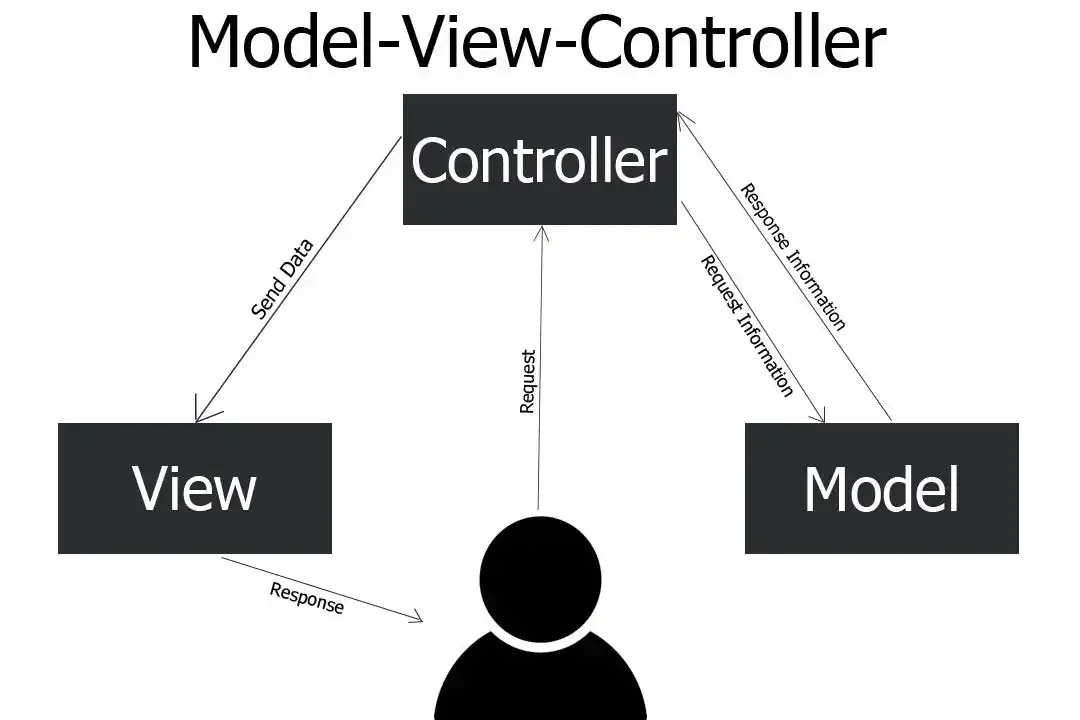
\includegraphics[width=0.8\linewidth]{lib/Arquitetura MVC.jpg}
      \caption{Arquitetura MVC}
      \label{fig:MVC}
\end{figure}

\begin{itemize}
      \item \textbf{\textit{Model} (Modelo)}: Representa os dados e a lógica de negócios subjacente, independentemente de como eles são apresentados ou manipulados. No contexto desta API de pôquer, o \textit{Model} encapsula entidades como Jogador, Mão de Cartas, Aposta e Rodada, gerenciando regras do jogo (ex.: validação de apostas válidas, cálculo de probabilidades via Monte Carlo) e persistência de dados (ex.: banco de dados para histórico de mãos). O \textit{Model} notifica as outras camadas sobre mudanças de estado, garantindo que a integridade dos dados seja mantida sem interferência de interfaces ou controles. De acordo com \citeonline{gamma1994}, o \textit{Model} é ``o coração da aplicação'', focado em abstrações do domínio problemático, o que facilita testes unitários e reutilização em diferentes contextos.

      \item \textbf{\textit{View} (Visão)}: Responsável pela apresentação e formatação dos dados para o usuário ou sistema externo, sem conter lógica de negócios. Em uma \gls{API} \textit{RESTful} como esta, a \textit{View} pode ser implementada como respostas \gls{JSON} formatadas (ex.: \textit{endpoint }\texttt{/jogo/\{id\}/estado} retornando o status atual da rodada em formato legível), templates \gls{HTML} para dashboards de simulação ou integrações com \textit{front-ends web}. A \textit{View} observa o \textit{Model} e se atualiza automaticamente via mecanismos de observador, conforme descrito no mesmo livro do \citeonline{gamma1994}. Isso assegura que alterações no \textit{Model} (ex.: nova aposta realizada) sejam refletidas imediatamente na saída, promovendo interfaces flexíveis e múltiplas \textit{views} para o mesmo conjunto de dados.

      \item \textbf{\textit{Controller} (Controlador)}: Atua como intermediário, processando entradas do usuário (ex.: requisições \gls{HTTP} POST para ações como ``apostar'' ou ``fold'') e orquestrando interações entre \textit{Model} e \textit{View}. No pôquer AI, o \textit{Controller} gerencia fluxos como inicialização de rodadas, chamadas à rede neural para decisões e execução de simulações Monte Carlo, direcionando atualizações no \textit{Model} e renderizando a \textit{View} apropriada.
            \citeonline{reenskaug1979} enfatizava que o \textit{Controller} ``interpreta comandos do usuário e atualiza o \textit{Model}'', evitando que a \textit{View} ou \textit{Model} lidem diretamente com inputs, o que reduz complexidade e facilita manutenção.
\end{itemize}

Essa tríade do \gls{MVC} permite ciclos unidirecionais eficientes: o usuário interage via \textit{Controller}, que modifica o \textit{Model}, que notifica a \textit{View} para atualização. Vantagens incluem escalabilidade (fácil adição de novas \textit{views}), testabilidade (camadas isoladas) e manutenção (mudanças em uma camada não afetam as outras), como validado em \textit{frameworks} modernos como \textit{Spring} \gls{MVC} (Java), Django (Python) e Laravel (PHP)\citeonline{rails2004}. Priorizando esses princípios, a arquitetura da \gls{API} define módulos específicos para o gerenciamento das etapas do jogo, execução de simulações Monte Carlo e integração com a rede neural para tomada de decisão e identificação de comportamentos automatizados. Essa estrutura modular isola funcionalmente cada componente --- \textit{Model} para lógica de pôquer, \textit{Controller} para \textit{endpoints} \gls{API} e \textit{View} para saídas, facilitando manutenção, depuração e expansões futuras.

Além disso, a arquitetura proposta contempla mecanismos de interface entre as camadas \gls{MVC}, assegurando comunicação eficiente e intercâmbio consistente de dados entre simulação estatística e aprendizado de máquina. Foram adotadas práticas de normalização de dados, controle de versionamento de \textit{endpoints} (ex.: \texttt{/v1/jogo/\{id\}}) e injeção de dependências para acoplamento frouxo, garantindo estabilidade e compatibilidade.

Essa etapa fundamenta a integridade técnica de todo o projeto, estabelecendo uma base sólida para fases subsequentes de testes, documentação e integração, ao mesmo tempo em que proporciona clareza estrutural e favorece a reprodutibilidade da pesquisa no contexto acadêmico.

\section{Inteligência artificial e aprendizado por reforço}
O termo inteligência artificial é extremamente amplo, o mesmo pode ser categorizado de várias maneiras diferentes, por exemplo: um inimigo que persegue o jogador em um jogo virtual é um tipo de inteligencia artificial. Mas o nicho que será abordado será o de \textit{Machine Learning}, que consiste em um sistema computacional aprender a executar uma ação, ou conjunto de ações, como é citado em \citeonline{sutton2018rl} pode ser entendido como uma criança aprendendo a brincar, ela faz movimentos aleatórios até entender quais movimentos se enquadram melhor para a brincadeira.
Para isso tomamos o modelo de aprendizado, já que o mesmo se enquadra melhor para a criação de uma agente capaz de jogar o Texas Hold'Em, dito isto, o agente pode ser baseado em três tipos de aprendizado de máquina, como destacado em \citeonline{russell2010artificial}, sendo alguns deles os seguintes:
\begin{itemize}
      \item \textbf{Supervisionado:} O agente observa padrões e/ou entradas e saídas que são disponibilizadas para que o mesmo aprenda da melhor maneira como usar aqueles dados para executar suas ações;

      \item \textbf{Não-supervisionado:} O agente trabalha sem necessariamente receber dados para complementar o modelo, como por exemplo um agente de tráfego de táxi, usando um modelo de aprendizado não supervisionado, ele pode usar diretrizes que o mesmo "percebeu" para ditar "Dias com tráfego bom" ou "Dias com tráfego ruim";

      \item \textbf{Aprendizado por reforço:} O agente aprende por uma série de recompensas ou penalidades, como o agente utilizado neste trabalho é baseado em um aprendizado de máquina por reforço, a maneira do próprio receber as recompensas e punições é feita por conta das fichas do poquêr, sendo ganhar fichas uma recompensa e perder uma penalidade.

\end{itemize}

Tendo os diferentes tipos de aprendizado mencionados, e como dito acima, o selecionado para este trabalho é um aprendizado de máquina por reforço, dado tal explicação cabe explicar os componentes que compõem um aprendizado por reforço, sendo eles:

\begin{itemize}
      \item \textbf{O agente:} É a inteligência artificial propriamente dita, o agente toma as decisões baseadas no ambiente em que o mesmo está enquadrado;

      \item \textbf{O ambiente:} Se trata de onde o agente vai trabalhar, no caso deste trabalho, se referencia à mesa de poquêr Texas Hold'Em, seguindo as regras estabelecidas do jogo;

      \item \textbf{O estado:} Pode ser dito como os elementos que estão à disposição do agente, e que neste caso, são váriaveis dependendo do momento do ambiente, neste caso as fichas e as cartas tomam o papel de estado;

      \item \textbf{A ação:} É definida como as ações que o agente pode tomar para obter o melhor resultado possivel, neste caso temos as seguintes ações: Fold, call e raise;

      \item \textbf{A recompensa:} Como o aprendizado utilizado é o aprendizado por reforço, o sistema de recompensa é essencial para moldar o agente da melhor maneira possivel, no caso deste trabalho o sistema de recompensa se baseia no lucro ou prejuízo de fichas, sengo ganhar fichar uma recompensa, enquanto perder fichas, ou deixar de ganhar, gera uma penalidade.
\end{itemize}

\section{Método de Monte Carlo aplicado a uma rede neural jogadora de pôquer}

O método de Monte Carlo é uma classe de técnicas numéricas baseadas em amostragem aleatória para estimar quantidades de interesse em problemas cuja solução analítica é inviável ou extremamente custosa. Historicamente, o método foi formalizado na década de 1940 no contexto do Projeto Manhattan em Los Alamos, quando Stanislaw Ulam e John von Neumann passaram a utilizar amostragens aleatórias para resolver problemas complexos de transporte de nêutrons e física nuclear, em substituição a cálculos combinatórios e integrais de alta dimensionalidade \citeonline{leonelli2021montecarlo}. O nome ``Monte Carlo'' foi sugerido por Nicholas Metropolis em referência ao famoso cassino de Mônaco, ressaltando a analogia com experimentos de sorteio e jogos de azar.

De forma geral, o objetivo do método de Monte Carlo é aproximar uma quantidade esperada, como uma integral ou esperança matemática, por meio da média de amostras geradas aleatoriamente. Dado um vetor aleatório \(X\) com distribuição \(p(x)\) e uma função de interesse $ f(x) $, deseja-se estimar a esperança

$$\mu = \mathbb{E}[f(X)] = \int_{-\infty}^{\infty} f(x)\, p(x)\, dx$$

Em muitos casos, essa integral não admite forma fechada ou é impraticável de calcular diretamente, especialmente em espaços de alta dimensão. O método de Monte Carlo substitui então essa integral pela média amostral
$$\hat{\mu}_N = \frac{1}{N} \sum_{i=1}^{N} f(X_i)$$
em que \(X_1, X_2, \dots, X_N\) são amostras independentes e identicamente distribuídas segundo \(p(x)\). Pelo Teorema da Lei dos Grandes Números, \(\hat{\mu}_N\) converge quase certamente para \(\mu\) quando \(N \to \infty\), e o Erro Padrão da estimativa diminui aproximadamente com a ordem de \(1/\sqrt{N}\) \cite{rubinstein2008simulation}. Essa propriedade torna o método de Monte Carlo particularmente útil para problemas de alta complexidade, onde métodos determinísticos teriam custo proibitivo.

Do ponto de vista prático, um algoritmo básico de Monte Carlo para estimar \(\mu\) pode ser descrito em três passos \cite{rubinstein2008simulation}:
\begin{enumerate}
      \item Gerar \(N\) amostras pseudoaleatórias \(X_1, X_2, \dots, X_N\) a partir da distribuição alvo \(p(x)\) ou de uma distribuição equivalente (por exemplo, via transformações, amostragem por rejeição ou métodos de cadeia de Markov).
      \item Avaliar a função de interesse \(f(X_i)\) para cada amostra gerada.
      \item Calcular a média amostral \(\hat{\mu}_N\) como estimativa da quantidade de interesse, juntamente com estimativas de variância e intervalos de confiança.
\end{enumerate}
Rubinstein e Kroese destacam que, embora o método seja conceitualmente simples, boa parte da pesquisa em Monte Carlo concentra-se em aprimorar a geração de amostras e reduzir a variância das estimativas (por exemplo, via amostragem estratificada, variáveis antitéticas ou amostragem por importância) \citeonline{rubinstein2008simulation}.

\subsection{Aplicação do método de Monte Carlo em jogos e pôquer}

Jogos de cartas como o pôquer são domínios clássicos para aplicação de Monte Carlo, pois envolvem incerteza combinatória (cartas ocultas, cartas futuras), múltiplos agentes e grandes espaços de estados. Em pôquer Texas Hold'em, por exemplo, um jogador conhece apenas suas cartas privadas e as cartas comunitárias já reveladas, mas desconhece as cartas dos oponentes e as cartas que ainda serão abertas. Isso torna difícil calcular exatamente a probabilidade de vitória ou o valor esperado de uma ação (pagar, aumentar, desistir) em tempo real.

O método de Monte Carlo é empregado para contornar essa dificuldade por meio de simulações do futuro da mão. A ideia básica é:
\begin{enumerate}
      \item Fixar o estado atual da mão: cartas próprias do agente, cartas comunitárias já reveladas, ações anteriores dos jogadores e tamanho dos potes.
      \item Amostrar aleatoriamente, muitas vezes, as cartas ocultas dos oponentes e as cartas futuras que ainda serão reveladas, respeitando o baralho remanescente (ou seja, sem reposição e sem conflitos com cartas já visíveis).
      \item Para cada cenário simulado, completar a mão até o final (showdown ou desistências) e avaliar o resultado: vitória, derrota, empate, lucro ou prejuízo monetário.
      \item Estimar, por meio da média dos resultados simulados, a probabilidade de vitória ou o valor monetário esperado (EV) de uma ação específica.
\end{enumerate}

Diversos trabalhos em pôquer computacional adotam variações desse esquema, tanto para avaliar a força de uma mão quanto para apoiar decisões estratégicas \citeonline{kleij2010thesis,vdBroeck2009mcts,heuristic2015poker}. Por exemplo, Van der Kleij construiu um jogador de pôquer computacional que utiliza busca em árvore por Monte Carlo, \gls{MCTS}, combinada com modelagem de oponentes para estimar valores esperados de ações em diferentes estágios do jogo \citeonline{kleij2010thesis}. Em outro estudo, Van den Broeck e colaboradores aplicam \gls{MCTS} em pôquer no-limit, utilizando simulações para explorar o espaço de decisões possíveis e discretizar tamanhos de aposta, reduzindo o custo computacional sem perder competitividade \cite{vdBroeck2009mcts}. Esses trabalhos demonstram que, mesmo em jogos de informação imperfeita, o uso sistemático de simulações aleatórias permite aproximar o valor das ações de forma eficaz.

Em contextos mais heurísticos, Monte Carlo também é amplamente utilizado para validar estratégias ou heurísticas de decisão em pôquer. Por exemplo, estudos utilizam simulações de centenas de milhares ou milhões de mãos para estimar a probabilidade de ocorrência de determinados tipos de mãos ou para verificar o desempenho de regras fixas de jogo ao longo do tempo \citeonline{heuristic2015poker}. Essa mesma lógica de simulação extensiva é diretamente aproveitada em arquiteturas de inteligência artificial, nas quais a estimativa robusta de probabilidades e valores esperados é um insumo fundamental para o treinamento de modelos.

\subsection{Integração do método de Monte Carlo com redes neurais para pôquer}

No contexto desta pesquisa, o método de Monte Carlo é empregado como um mecanismo de estimação estatística que gera alvos ou sinais de treinamento para uma rede neural projetada para jogar pôquer. A integração entre Monte Carlo e aprendizado de máquina segue a linha de trabalhos em aprendizado por reforço (Reinforcement Learning), nos quais estimativas de retorno obtidas a partir de episódios completos são utilizadas para atualizar funções de valor e políticas.

Em termos conceituais, a rede neural recebe como entrada uma representação de estado do jogo (por exemplo, codificação das cartas próprias, cartas comunitárias, posição na mesa, tamanho dos potes, histórico recente de apostas e características dos oponentes) e produz como saída:
\begin{itemize}
      \item estimativas de valor, representando o valor esperado da posição atual (por exemplo, em unidades monetárias ou em probabilidade de vitória); e/ou
      \item distribuições de probabilidade sobre ações (por exemplo, dobrar, pagar, aumentar), representando uma política estocástica de jogo.
\end{itemize}
Para treinar essa rede, o método de Monte Carlo é utilizado em duas frentes principais:

\subsubsection{Geração de rótulos (targets) a partir de simulações}

Uma abordagem direta consiste em usar simulações de Monte Carlo para rotular estados com estimativas de valor ou probabilidade de vitória. O procedimento típico é:
\begin{enumerate}
      \item Selecionar um conjunto de estados de pôquer (reais ou gerados artificialmente).
      \item Para cada estado, executar um grande número de simulações Monte Carlo, amostrando cartas ocultas dos oponentes e cartas futuras, e jogando a mão até o fim sob uma política fixa ou sob um modelo de oponentes.
      \item Calcular, para cada estado, a média dos resultados simulados (por exemplo, lucro líquido médio ou probabilidade estimada de vitória).
      \item Utilizar esses valores médios como alvos supervisionados para treinar a rede neural, minimizando uma função de perda adequada (como erro quadrático médio para valores ou entropia cruzada para probabilidades).
\end{enumerate}
Essa estratégia transforma o problema em um cenário de aprendizado supervisionado onde Monte Carlo fornece um especialista para a rede, à semelhança do que \citeonline{sutton2018rl} discutem para métodos de Monte Carlo em aprendizado por reforço, nos quais o retorno total observado em um episódio serve como alvo para a função de valor.

\subsubsection{Métodos de Monte Carlo em aprendizado por reforço}

Outra forma de integração é empregar diretamente métodos de Monte Carlo em aprendizagem por reforço, em que a própria interação da rede com um ambiente simulador de pôquer gera episódios de jogo. Nesse cenário:
\begin{itemize}
      \item Cada episódio corresponde a uma sequência de estados, ações e recompensas (por exemplo, ganhos e perdas em fichas).
      \item Ao final do episódio, calcula-se o retorno total \(G_t\) a partir de cada estado \(s_t\):
            $$G_t = \sum_{k=t+1}^{T} \gamma^{k-t-1} R_k,$$
            em que \(R_k\) é a recompensa na etapa \(k\), \(\gamma \in [0, 1]\) é o fator de desconto e \(T\) é o tempo final do episódio.
      \item Esses retornos \(G_t\) são utilizados para atualizar os parâmetros da rede, seja como alvos para uma função de valor \(V(s)\), seja como sinal de reforço para ajustar uma política parametrizada \(\pi_\theta(a|s)\).
\end{itemize}
\citeonline{sutton2018rl} mostram que tais métodos de Monte Carlo permitem aprender diretamente a partir da experiência, sem a necessidade de um modelo completo das dinâmicas do ambiente, o que é particularmente atraente em domínios complexos como o pôquer, em que a modelagem exata dos oponentes e das distribuições de cartas é difícil. Na prática, pode-se combinar simulações de Monte Carlo com técnicas como busca em árvore \gls{MCTS} ou amostragem de políticas para explorar as consequências de diferentes ações antes de atualizá-las na rede neural.

\subsection{Aspectos práticos e considerações metodológicas}

A aplicação do método de Monte Carlo em pôquer associado a redes neurais envolve algumas decisões metodológicas importantes:
\begin{itemize}
      \item \textbf{Número de simulações (\(N\))}: Há um compromisso entre custo computacional e precisão estatística. Valores de \(N\) muito baixos resultam em estimativas ruidosas, enquanto valores muito altos aumentam o tempo de treinamento. Em geral, escolhe-se \(N\) de forma a garantir erros padrão aceitáveis para as estimativas de valor, muitas vezes com base em experimentos preliminares como dito por \citeonline{rubinstein2008simulation}.
      \item \textbf{Modelagem de oponentes}: Em jogos de informação imperfeita, as simulações devem refletir crenças realistas sobre o comportamento dos oponentes. Trabalhos em pôquer computacional utilizam modelos paramétricos de oponentes, aprendidos a partir de dados, para amostrar ações e cartas de forma consistente com estilos de jogo observados por \citeonline{kleij2010thesis,vdBroeck2009mcts}.
      \item \textbf{Representação de estados}: A qualidade das estimativas de Monte Carlo depende também da expressividade da representação utilizada na rede neural. Entradas que resumem adequadamente a informação relevante (por exemplo, tamanhos relativos de pilha, posição, textura do bordo e histórico de ações) favorecem o aprendizado de padrões estáveis a partir dos retornos simulados.
      \item \textbf{Redução de variância}: Técnicas clássicas de redução de variância podem ser adaptadas ao contexto de pôquer, por exemplo, estratificando simulações por tipo de mão inicial ou por determinadas configurações de bordo, de modo a obter estimativas mais precisas sem necessariamente aumentar \(N\) como notado por \citeonline{rubinstein2008simulation}.
\end{itemize}

Dessa forma, o método de Monte Carlo funciona como um elemento estruturante, fornecendo a base estatística para a estimativa de probabilidade de vitória, valor esperado de ações e retornos de aprendizado por reforço.

\section{Redes neurais artificiais e Q-Learning}

Uma \gls{RNA} emula o funcionamento do cerébro humano, neste aspecto, há varias formas de moldar uma \gls{RNA}, a que será citada será uma rede neural artificial perceptron multicamadas, como dito em \citeonline{bengio2017deep}, a mesma pode ser definida como uma função que mapeia um conjunto de entradas e retorna uma saída, utilizando para isso, neurônios, que servem para definir as saídas baseadas nas entradas, pesos, que são paramêtros passados para os neurônios para tomarem a melhor decisão e funções de ativação que, como o nome se refere, ativa os neurônios.

O Q-Learning é um algoritmo de aprendizado por reforço que associa valores de qualidade, \textit{Q-Values}, às ações disponiveis em determinado estado, de modo a estimar a melhor decisão. O Q-Learning trabalha usando a Q-Table, que consiste em uma tabela que suas linhas são todos os estados possíveis do jogo, enquanto as colunas são todas as ações possíveis, a rede verifica o estado e confere qual ação tem o maior Q-Value e executa a devida ação.

Para calcular o valor ideal do Q-Value, como citado por \citeonline{mnih2015human},é utilizada a fórmula de Bellman, cuja é a seguinte:
$$Q_{i+1}(s, a) = r + \gamma \max Q_i(s', a')$$
Tal fórmula calcula o Q-Value, cada termo significa o seguinte:
\begin{itemize}
      \item $Q_{i+1}(s, a)$: Significa o valor a ser calculado, onde o \textit{s} representa o estado que o agente se encontra, enquanto o \textit{a} representa a ação a ser tomada, o \textit{i+1} representa o novo valor a ser adicionado;
      \item \textit{r}: Representa a recompensa imediata por tomar tal ação;
      \item $\gamma$: Representa o fator de desconto, variando entre 0 e 1, sendo 0 quando o agente leva em consideração apenas a recompensa imediata(\textit{r});
      \item $\max Q_i(s', a')$: Esta função representa o maior Q-Value possível, tomando o estado futuro (\textit{s'}) tomando a melhor ação possível (\textit{a'}).
\end{itemize}

Entretanto um algoritmo de Q-Learning tradicional funciona perfeitamente com jogos mais simples e com menos ações e estados a serem verificados, jogos como jogo da velha ou labirintos são exemplos simples para se utilizar o Q-Learning tradicional, porém o Texas Hold'Em, por conta da quantidade de combinações de cartas, tamanho do pote, quantidade de fichas do jogador e ações a serem tomadas, criaria uma tabela que beiraria a infinidade de estados que poderiam ser tomados, tornando ineficaz e praticamente impossível a criação de uma Q-Table para um jogo de pôquer, tendo em vista que nenhum computador moderno teria capacidade de memória para alocar uma tabela tão extensa.


\section{Deep Q-Network}
O Deep Q-Network é uma variação do algoritmo de Q-Leaning padrão, o mesmo é usado quando a quantidade de estados beira o infinito, já que o mesmo usa de uma rede neural para fazer a predição do Q-Value.

Como citado anteriormente, esta abordagem não é eficiente já que é calculada sem nenhuma generalização, sendo assim, o Deep Q-Network foi criado para que fosse possível que a rede neural fizesse a predição sem necessidade de criar uma tabela grande demais até mesmo para ser alocada na memória, assim podendo usar uma equação para se calcular o valor aproximado do Q-Value, usando a equação:

$$L_i(\theta_i) = \mathbb{E}_{\underbrace{(s,a,r,s') \sim U(D)}_{\text{Exp. Replay}}} \left[ \left( r + \gamma \underbrace{\max_{a'}}_{\text{Alvo}} Q(s', a'; \theta_i^-) - \underbrace{Q(s, a; \theta_i)}_{\text{Predição}} \right)^2 \right]$$

Esta é uma fórmula de perda, descrita por \citeonline{mnih2015human}, que pode ser desmembrada e entendida como:

\begin{itemize}
      \item $L_i(\theta_i)$: é a taxa de perda na iteração \textit{i}, considerando os pesos atuais $\theta_i$ da rede neural;
      \item  $ \mathbb{E}_{(s,a,r,s') \sim U(D)} $: Se refere ao \textit{Experience Replay}, que são jogos anteriores guardados na memória;
      \item $ r + \gamma {\max_{a'}} Q(s', a'; \theta_i^-)$: É a equação de Bellman, porém utilizando iterações passadas otimizadas pela fórmula de perda, representadas por $\theta_i^-$, sendo utilizada como alvo;
      \item $ Q(s, a; \theta_i) $: Representa a predição feita de forma cega pelo agente, utilizando os pesos $\theta_i$;
      \item Sendo a diferença entre o alvo e a predição elevados ao quadrado, para evitar números negativos, e dar maior peso a resultados ruins.
\end{itemize}

O Deep Q-Network foi desenvolvido por \citeonline{mnih2015human} para ensinar uma Inteligencia artificial para jogar Atari, tornando-se um marco histórico para o desenvolvimento de Redes Neurais utilizando o Q-Learning.

\section{Exploração vs. Explotação (Epsilon-Greedy)}

O agente necessita aferir a melhor jogada possível do Texas Hold'Em, para isso ele deve explorar suas opções de jogada, o mesmo inicialmente não tem conhecimento para determinar a melhor jogada possível, logo o agente deve escolher aleatoriamente sua jogada, antes de conseguir explotar as melhores jogadas possíveis.

Para isso, foi usada a tática \textit{$\epsilon$ -Greedy}(Epsilon-Guloso), como descrita em \citeonline{sutton2018rl}, o $\epsilon$ -Greedy consiste em uma tática em que o coeficiente de exploração $\epsilon$ determina a aleatoriedade das ações, no caso deste trabalho, o mesmo é iniciado em 1.0, determinando exploração total, ou seja, uma ação completamente aleatória, que vai decaindo ao decorrer das jogadas, chegando próximo de 0.0, assim maximizando a explotação.

\section{Replay de Experiência (Experience Replay)}

Pela extensa quantidade de estados que o Texas Hold'Em pode tomar, alguns estados se tornam semelhantes entre si, o que pode ocasionar um ótimo local para a Rede Neural, isso é denotado por \citeonline{mnih2015human}, quando é citado que casos semelhantes "viciam" nas ações, tornando o agente enviesado.

Para contornar este problema foi utilizado o \textit{Experience Replay}(Replay de experiência), também citado em \citeonline{mnih2015human}, o Experience Replay consiste em criar lotes de memórias aleatórias do passado para serem usados antes do agente decidir a jogada, servindo como parte do treino, e assim evitando enviesamentos do agente, deixando o mesmo mais robusto e mais assertivo com a proposta do jogo.
\chapter{Trabalhos Relacionados}
\label{cap:trabalhos-relacionados}

\section{Abordagens baseadas em busca}

Antes de redes neurais mais profundas serem amplamente utilizadas para produção de projetos envolvendo o \textit{Texas Hold'Em}, eram utilizadas abordagens mais voltadas para busca em árvore, como feito por \citeonline{kleij2010thesis} e por \citeonline{vdBroeck2009mcts}, que utilizaram o algoritmo de \textit{Monte Carlo} para explorar os estados do jogo, porém como ambos focavam majoritariamente na modelagem e busca em árvore de maneira mais bruta, enquanto este trabalho é mais focado na tomada de decisões em si, porém o \textit{Monte Carlo} é usado de forma semelhante nas fase de \textit{Pré-Flop} e de \textit{Pós-Flop} para calcular o valor de equidade.

\section{Avanço em \textit{Deep Reinforcement Learning}}

Com o passar do tempo, técnicas de Aprendizado por Reforço Profundo se tornaram mais utilizadas para desenvolvimento de agentes inteligentes capazes de jogar o \textit{Texas Hold'Em}, como feito por \citeonline{moravvcik2017deepstack}, que desenvolveu um agente capaz de vencer jogadores profissionais de poquêr \textit{Heads-Up}, outra categoria do jogo quem consiste em um contra um direto, utilizando clusters poderosos carregados de dados, enquanto este trabalho é mais focado na intuição dos jogos.

Enquanto a maioria dos trabalhos realizados para criação de agentes para jogar poquêr jogam apenas a categoria \textit{Heads-Up}, e enfrentam inúmeros problemas de ótimo local, assim como \citeonline{mnih2015human} tentou desenvolver um agente utilizando apenas uma \gls{DQN} puro para jogar o \textit{Texas Hold'Em}, mas atingiu ótimos locais de desistências infinitas assim como este trabalho, tendo isso em vista \citeonline{heinrich2016deep} desenvolveu um agente capaz de jogar \textit{Texas Hold'Em} utilizando táticas para contornar as fraquezas do \gls{DQN}, enquanto a tática utilizada neste trabalho foi a de penalidade por jogar passivamente.

Também pode ser citado o artigo de \citeonline{brown2019superhuman} que desenvolveu um agente que se sobressaiu em uma mesa com 6 jogadores, demonstrando um domínio completo sobre ambientes multi-jogadores, o agente jogava de maneira que não permitia que os outros jogadores explorassem suas falhas, tendo um comportamento similar ao agente desenvolvido neste trabalho, que explora a falha dos outros jogadores para tomar as melhores decisões possíveis.

\section{Diferença arquitetural}

Enquanto os trabalhos citados anteriormente dispunham de um extenso maquinário para o desenvolvimento dos agentes, este trabalho se voltou mais para o fator de exploração do agente, fazendo com que o próprio aprendesse com suas próprias ações, além de utilizar modulagem de recompensa para deixar o agente mais preciso, o penalizando por fazer uma jogada desnecessariamente passiva, ou o recompensando por fazer uma jogada embasadamente agressiva, fazendo com que o jogador tenda a seguir mais fielmente a dinâmica do \textit{Texas Hold'Em}.

Também pode ser citada a questão de desempate, que costuma ser resolvida por buscas em árvores complexas e mais custosas, este projeto desenvolveu um motor de base 15 capaz de efetuar os desempates de forma concisa e coerente, deixando o programa relativamente mais rápido. A linguagem utilizada para o desenvolvimento também é diferente da maioria utilizada, já que foi utilizado o \textit{JavaScript}, utilizando do \textit{TensorFlow.js} e \textit{Node.js} como uma alternativa no lugar da comumente usada \textit{Python}.



\chapter{Metodologia}
\label{chap:metodologia}

\section{Tecnologias e Ferramentas Utilizadas}

A linguagem utilizada para este trabalho foi a \textit{JavaScript}, usando os recursos do \textit{Node.js}, já que foram executados longos \textit{loops} para simular milhares de mãos de \textit{Texas Hold'Em}. Tendo em vista que a quantidade de iterações poderia gerar travamentos na execução, as funções assíncronas do \textit{Node.js} \textit{(await/assync)} tornavam a execução do programa mais eficiente.

Para desenvolvimento da Rede Neural, foi utilizado o \textit{TensorFlow.js}, dispensando a necessidade de fazer uma conexão entre \textit{JavaScript} e \textit{Python} caso fosse usado apenas o \textit{TensorFlow} tradicional, sendo utilizado como referenciado por \citeonline{smilkov2019tensorflow}. Tendo em vista que o \textit{TensorFlow.js} tem funções nativas de \gls{DQN}, a mesma foi a mais adequada para o trabalho.

A plotação gráfica foi feita utilizando do \textit{Chart-Js-Node-Canvas}, \gls{API} que permite a criação dos gráficos, sendo utilizada para plotar o desempenho do agente, levando como parâmetro o ganho/perda de fichas, também representando a queda do $\epsilon$.

\section{Arquitetura do ambiente e motor de regras}

\subsection{Estrutura \texorpdfstring{\gls{MVC}}{MVC}}
Este trabalho é todo arquitetado utilizando o padrão de arquitetura \gls{MVC}, como é possível verificar no repositório de \citeonline{grangeiro2026poker}. A pasta \textit{Models} comporta as classes referentes ao \textit{Texas Hold'Em}, sendo elas a classe ``carta'' que representa as cartas do baralho utilizadas no pôquer, contendo o Naipe e o Valor da carta, e a classe ``jogador'' representa o agente, que contém as cartas disponíveis para o jogador, seu \textit{Stack} e a ação que o jogador vai tomar.
A pasta \textit{controllers} possui o controlador responsável por gerenciar as fases de apostas, sendo elas as descritas no código como:
\begin{lstlisting}[language=JavaScript, caption={Fases gerenciadas pelo jogoController.js}, label={cod:fases}]
const fases = [
        { nome: "Pre-Flop", cartas: 0 },
        { nome: "Flop", cartas: 3 },
        { nome: "Turn", cartas: 1 },
        { nome: "River", cartas: 1 }
    ];
\end{lstlisting}
A pasta \textit{Services} vai conter toda a parte estatística e da inteligência do agente, podendo ser considerada o cerébro das atividades do projeto, contendo todas as funções referentes ao baralho, a Inteligencia Artificial, os gráficos, as combinações e as estatísticas geradas pelo \textit{Monte Carlo}.
Por fim, a pasta \textit{Views} gerencia aquilo referente ao que o usuário vê durante o processamento do programa, no caso deste trabalho, controla a barra de carregamento que pode ser vista no terminal de comandos, além como as funções responsáveis por escrever informações em um arquivo de texto e uma função responsável por escrever as cartas de maneira mais compreensível para o usuário.

\subsection{Motor de avaliação - Base 15}

Um dos principais desafios para se modular as regras do pôquer são a valorização das jogadas, porém é possível superar esse desafio usando lógica simples, dando valores de força para as jogadas, entretanto cai-se em outra barreira, os empates são ocasiões incomuns, mas que são um grande desafio de serem resolvidos usando uma simples lógica de valores para as jogadas. Mesmo que o pôquer disponha do \textit{Kicker}, sendo necessário verificar qual categoria se sobressai, para seres humanos é fácil distinguir quais pares são maiores que outros, por exemplo, mas para o computadores, se o par tem sempre peso 2, independete do valor dos pares, eles serão iguais.

Para contornar isso, foi elaborado um sistema de \textit{score}(pontuação) de base 15, tomando o Ás como valor 14, a base 15 supre todas as necessidades do sistema, garantindo que não haverão possibilidades maiores que o ás, para calcular esse \textit{score} é usada a seguinte formula:

$\text{Score} = (\text{Categoria} \cdot 15^5) + \sum_{i=1}^{5} \left( \text{Carta}_i \cdot 15^{5-i} \right)$

Esta fórmula calcula o score multiplicando o valor da categoria da jogado por $15^5$, sucedido pela soma das 5(cinco) cartas que o jogador tem à sua disposição, cada uma multiplicada por uma exponenciação de base 15(quinze).
A função do código que faz esse cálculo se encontra no \textit{combinacaoService.js}, cuja é:

\newpage
\begin{lstlisting} [language=JavaScript, caption={Função de cálculo do Score}, label={cod:score}]
    const calcularScore=(categoria, v1=0, v2=0,v3=0, v4=0,
v5=0)= >{
        return categoria*759375 + v1*50625 + v2*3375 + v3*225
        + v4*15 + v5 ;
    };
\end{lstlisting}

Para melhor compreensão do motor base 15 e de como ele é utilizado de forma real no código, segue o exemplo de cálculo para a categoria \textit{Dois Pares}:

\begin{lstlisting} [language=JavaScript, caption={Função de score de Dois Pares}, label={cod:doispares}]
     if(pares.length>=2) {
        let k=kickers([pares[0], pares[1]]);
        return calcularScore(3, pares[0], pares[0], pares[1], pares[1], k[0]);
    }
\end{lstlisting}

Nesse caso, o primeiro paramêtro da função \textit{calcularscore} se refere a força da categoria, no caso de Dois pares a força é 3(três), seguido pelo par maior duas vezes como pode ser notado em \textit{pares[0], pares[0]} para ocupar os multiplicadores mais fortes, sendo esses $15^4$ e $15^3$, seguido pelos dois pares menores, que consequentemente recebem os multiplicadores mais fracos, e por fim o \textit{Kicker}, que consiste nas cartas de desempate, nesse caso sendo a última carta disponivel do agente.

Sendo assim, na rara ocasião que dois jogadores possuam Dois Pares cada um e o mesmo \textit{Kicker}, o programa é capaz de definir o que se sobressai, dando a vitória para o jogador com a maior jogada.

\section{Modelagem do agente inteligente (\textit{DQN})}

\subsection{Arquitetura e espaço de estados}

Tendo em vista que o \textit{TensorFlow.js} foi a \gls{API} selecionada para este trabalho, o mesmo foi arquitetado com duas camadas ocultas de 16 neurônios, tal quantidade foi escolhida por meio de tentativa e erro, menos neurônios deixavam o agente impreciso, mais deixavam a execução mais lenta, sem mudar significativamente os resultados, com ativação \gls{ReLU}, que cortam quaisquer números negativos que possam entrar na rede, além de uma camada de saída com 5 neurônios de ativação linear, já que o \textit{Q-Learning} retorna um score absoluto, ao invés de uma probabilidade, tudo isso pode ser denotado no seguinte trecho do código:

\begin{lstlisting}[language=JavaScript, caption={Camadas do modelo}, label={cod:camadas}]
    createModel(){
        const model=tf.sequential();
        model.add(tf.layers.dense({units: 16, inputShape: [4], activation: 'relu'}));
        model.add(tf.layers.dense({units: 16, activation: 'relu'}));
        model.add(tf.layers.dense({units: 5, activation: 'linear'}));
        model.compile({optimizer: 'adam', loss: 'meanSquaredError'});
        return model;
    }
\end{lstlisting}

Além disso, o estado do agente é composto por 4(quatro) parâmetros, sendo eles o \textit{equityMC}, que é o valor de equidade retornado pelo \textit{Monte Carlo}, o \textit{pote}, que consiste na quantidade de fichas já apostadas na rodada, a \textit{apostaParaCobrir} que representa quanto o agente deve pagar para continuar na rodada, por fim, o parâmetro \textit{minhasFichas} que diz quantas fichas disponíveis o jogador tem. Entretanto, o valor da equidade se encontra entre 0 e 1, enquanto os parâmetros baseados em fichas podem variar de 0 até 1000, sendo necessária uma normalização desses parâmetros, para não haverem conflitos no processamento do estado, é possível ver os parâmetros e a normalização no trecho a seguir:

\begin{lstlisting}[language=JavaScript, caption={Estado do jogador}, label={cod:estado}]
    obterEstado(equityMC, pote, apostaParaCobrir, minhasFichas){
        // Normalizacao basica para ajudar a rede
        return [equityMC, pote/1000, apostaParaCobrir/1000, minhasFichas/1000];
    }
\end{lstlisting}

\subsection{Espaço de ações}

Considerando que as apostas no \textit{Texas Hold'Em} são o fator mais importante para o jogo, é extremamente importante que o agente consiga executa-las de maneira consistente, entretanto, como no jogo tradicional as apostas tem valores extremamente imprecisos, podendo variar entre 1 até o todas as fichas disponíveis do jogador, e isso se tornaria um empecilho para o \textit{Q-Learning}, sendo assim, foi feita uma discretização das ações.

Como citado anteriormente, a rede neural possui 5 neurônios de saída, que podem ser ditos como as ações que o agente toma, sendo eles os seguintes:
\begin{itemize}
    \item \textit{Fold}: O agente desiste da mão;
    \item \textit{Check/call}: O agente paga as apostas que vem na mesa, ou passa a vez caso não tenham apostas à serem pagas;
    \item \textit{Raise Leve}: O agente adiciona mais 150 fichas na aposta que vem para ele pagar;
    \item \textit{Raise Forte}: O agente adiciona mais 300 fichas na aposta que vem para ele pagar;
    \item \textit{All In}: O agente aposta todas as suas fichas disponíveis.
\end{itemize}

\subsection{Modelagem das recompensas}

As recompensas são a principal forma de se treinar um agente por reforço. Seguindo as regras do \textit{Texas Hold'Em}, as recompensas podem ser dadas simplesmente pelo lucro ou prejuízo de fichas, entretanto apenas usar o lucro/prejuízo do agente pode encaminha-lo para ótimos locais, como dito por \citeonline{russell2010artificial}, um ótimo local é quando o agente ``descobre'' a melhor forma para o que ele aprendeu, mesmo que fuja do ótimo global, que seria a tomada de decisão ideal, no caso deste trabalho, o agente atingiu um ótimo local em que o mesmo sempre desistia de todas as mãos, assim ele não perdia fichas. Para contornar isso, foi utilizada a estratégia de \textit{Blinds}, que são apostas rotativas no \textit{Texas Hold'Em} que forçam o agente a apostar na primeira rodada, o que resolveu o ótimo local do \text{fold} na primeira fase, porém, o agente aprendeu que caso apenas desse \textit{Check}, também perderia o mínimo de fichas possiveis. Sendo assim, foi necessário a implementação de uma penalização por passividade, associado de uma bonificação por agressividade, como denonado por \citeonline{ng1999policy}, sendo feita como indicado na Figura 2:

\begin{figure}[htbp]
    \centering
    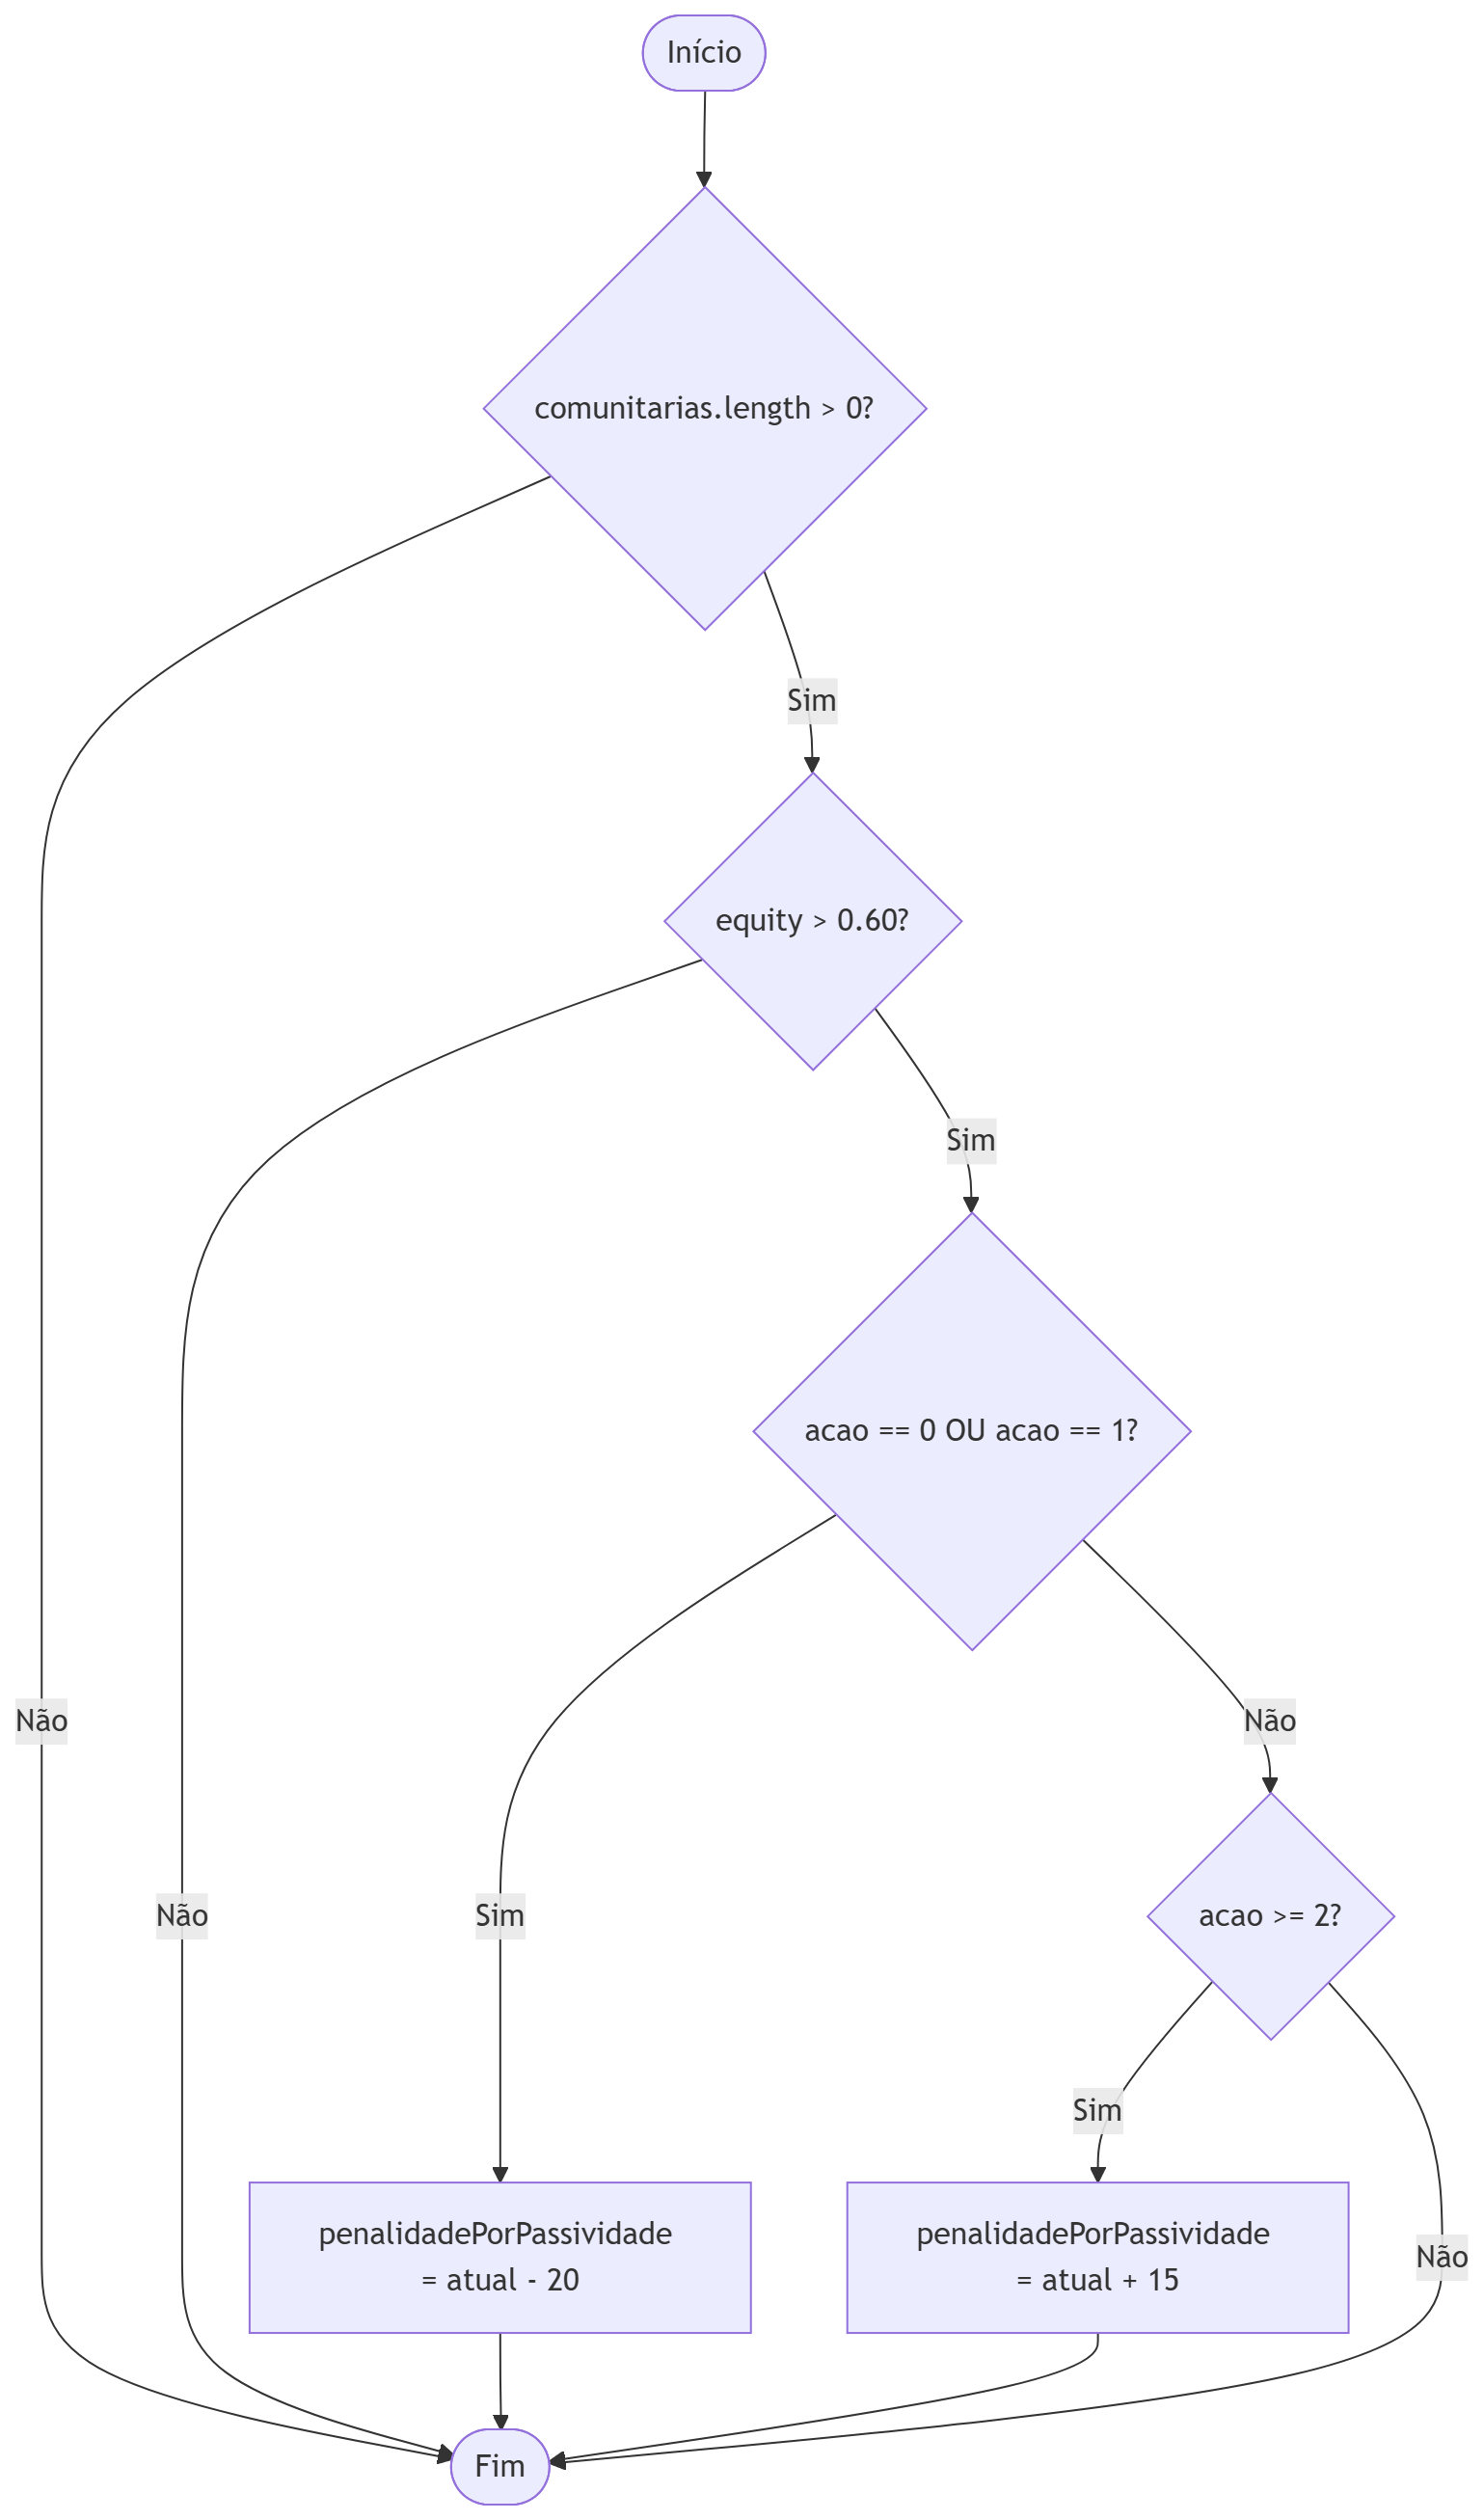
\includegraphics[width=0.5\linewidth]{lib/Fluxograma das penalidades.png}
    \caption{Fluxograma do sistema de penalidade por passividade: Autoria própria}
    \label{fig:desempenhoAgente}
\end{figure}

Como pode ser visto, caso o agente tenha um \textit{equity} superior a 60\%, o mesmo é penalizado em 20 pontos caso escolha a ação de \textit{Fold} ou de \textit{Check}, enquanto recebe uma bonificação de mais 15 quando faz uma jogada agressiva, como aumentar a aposta ou até mesmo dar \textit{all-in}.
Sendo assim, o agente evita os ótimos locais mencionados, além de deixar o sistema de recompensas mais robusto, fazendo que o agente seja mais assertivo conforme aprende a jogar o jogo

\section{Cenários de simulação e Treinamento}

\subsection{O ambiente da mesa}

O ambiente foi configurado para comportar 4 agentes que fazem o papel de jogador, cada um iniciando com um \textit{Stack efetivo}(fichas inicias) de 1000 fichas, com a existência do \textit{Small Blind} e do \textit{Big Blind}, sendo apostas obrigatórias rotativas que os jogadores são obrigados a pagar quando são selecionados, cobrindo todos os jogadores da mesa.

\subsection{A execução dos treinos}

O treinamento ocorre por grandes lotes contínuos de partidas, com exemplo de 10.000 mãos sendo feitas, cada mão podendo ser repetida pela \gls{RNA}, usando assim uma simulação em vários cenários, como descrito por \citeonline{leonelli2021montecarlo}, aplicando os \textit{Experience Replay} utilizando lotes de 32 memórias no final de todas as mãos.

\subsection{O decaimento do \textit{Epsilon}}

Sendo usado como fator de aleatoriedade nas primeiras mãos, já que o agente não sabe como jogar no inicio, o $\epsilon$ é iniciado em 1.0, definindo aleatoriedade total no começo das simulações, decaindo em 0.5\% a cada mão, chegando até o valor mínimo de 0.01 , esse decaimento é definido no seguinte trecho de código:

\begin{lstlisting}[language=JavaScript, caption={Variáveis responsáveis pelo controle do epsilon}, label={cod:varEpsilom}]
        this.epsilon=1.0;
        this.epsilonMin=0.01; 
        this.epsilonDecay=0.995; 
\end{lstlisting}

Tendo isso em vista, o $\epsilon$ é decrementado no fim de cada simulação da seguinte maneira:

\begin{lstlisting}[language=JavaScript, caption={Decaimento do epsilon}, label={cod:decaEpsilom}]
        if(this.epsilon>this.epsilonMin){
            this.epsilon*=this.epsilonDecay;
        }
\end{lstlisting}

\chapter{Resultados}
\label{chap:resultados}

\section{Validação do ambiente e do motor de regras}

Tomando um ambiente em que foram executadas 10.000 simulações de mãos do \textit{Texas Hold'Em}, cada mão sendo repetida 10 vezes, o motor de base 15 executou o trabalho de maneira consistente, classificando todos os jogos de fazer os desempates de maneira correta e robusta. Isso pode ser atestado observando o jogo 20 das simulações, que é o que consta no Apendice-a.

Esta simulação demonstra o funcionamento do motor base 15, já que o \textit{Jogador[0]} e o \textit{Jogador[2]} possuíam dois pares, porém o \textit{Jogador[0]} levou a vitória por pontuar mais, já que, seguindo a fórmula para o motor de desempate, o \textit{jogador[0]} pontuou 2.819.809 pontos, enquanto o \textit{jogador[2]} pontuou 2.819.098, uma diferença de 711 pontos, mesmo o \textit{Jogador[2]} possuindo um kicker de Ás, porém os pares do \textit{jogador[0]} eram superiores.

\section{Evolução na taxa de exploração}

\begin{figure}[htbp]
    \centering
    \caption{Decaimento do fator de exploração \textit{epsilon}($\epsilon$).}
    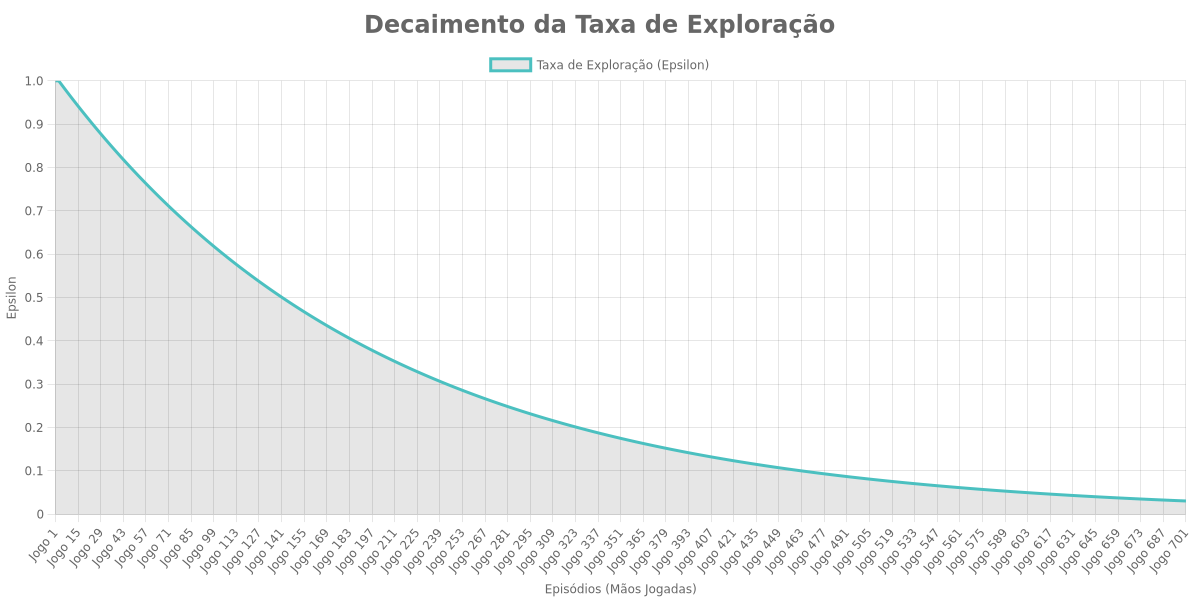
\includegraphics[width=0.8\textwidth]{lib/Decaimento epsilon.png}
    \label{fig:decaimentoEpsilon}

    \small{Fonte: Autoria própria}
\end{figure}

O gráfico demonstra o decaimento do fator de exploração \textit{epsilon} ($\epsilon$), sendo possível notar que a partir de por volta do jogo 700, a taxa de exploração é mínima, significando que o agente está jogando com tudo o que aprendeu, ao invés de apenas tomar ações aleatórias.

\section{Desempenho e lucro do agente}

Durantes as simulações, o agente a ser observado foi o responsável pelo \textit{Jogador[0]}. Para facilitar o entendimento e plotação gráfica, é possível verificar o lucro ou prejuízo do agente observado no seguinte gráfico:

\begin{figure}[htbp]
    \centering
    \caption{Desempenho do agente ao longo das simulações}
    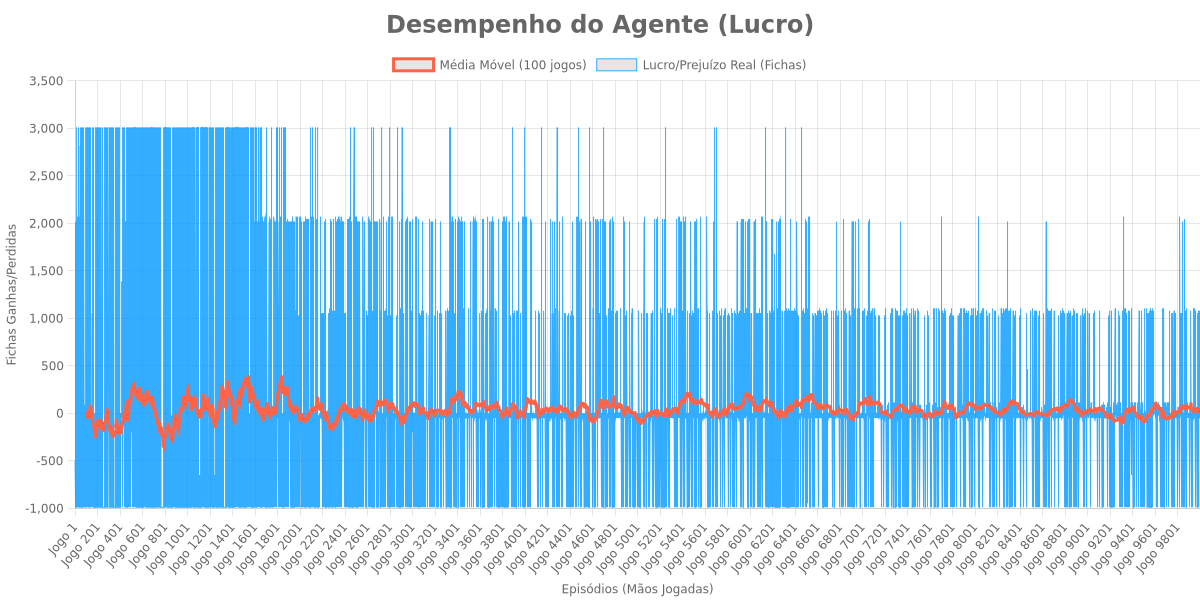
\includegraphics[width=0.97\linewidth]{lib/Desempenho do agente.png}
    \label{fig:desempenhoAgente}

    \small{Fonte: Autoria própria}
\end{figure}

A variância praticamente infinita de estados do \textit{Texas Hold'Em} gera um gráfico com grandes flutuações, porém é possível perceber que a flutuação de ganho e perda de fichas pelo agente cai drasticamente conforme as simulações, as primeiras simulações em que o agente está explorando e toma ações aleatórias a flutuação é maior que nas outras partes, que vão decaindo conforme a rede neural aprende a lidar melhor com os estados.
\chapter{Conclusões e Trabalhos Futuros}
\label{chap:conclusoes-e-trabalhos-futuros}

O principal objetivo deste trabalho era desenvolver um agente capaz de jogar o poquêr \textit{Texas Hold'Em}, utilizando de uma rede neural e algoritmos de predição, sendo assim, o objetivo foi alcançado por meio de uma rede neural utilizando aprendizado por reforço e o algoritmo de predição \textit{Monte Carlo}, o agente se mostrou coerente com o proposto, utilizando métodos de desempate robustos e complexos, enquanto eram evitados gargalos, aplicando o motor de pontuação de base 15, uma resolução matemática concreta e que se mostrou extremamente precisa na categorização de cada jogo possível do \textit{Texas Hold'Em}.

Entretanto, pela natureza continua e variável das apostas do \textit{Texas Hold'Em}, o \textit{Q-Learning} não viabiliza tal variação das apostas, já que tornaria os \textit{Q-Values} ainda mais complexos de serem aplicados, sendo assim foi necessário fazer uma discretização das apostas, não dando liberdade para o agente escolher o tamanho da aposta, limitando o mesmo a apenas cinco ações, sendo elas: \textit{Call/Check}, \textit{Raise} leve, \textit{Raise} forte, \textit{fold} e \textit{All-In}. Além de limitações performáticas matriciais, já que o \textit{Node.js} não é tão eficiente quando se trata de calculo de matrizes complexas. O programa também tem um ciclo de apostas fechado, não possibilitando um aumento cada vez maior das apostas, por exemplo, caso o último agente aposte uma quantia, o primeiro agente não é capaz de cobrir essa aposta, ou até mesmo aumenta-la.

Para trabalhos futuros pode-se sugerir a ideia de fazer a substituição do algoritmo de \gls{DQN} por algoritmos capazes de lidar com ações continuas de apostas, tornando o agente ainda mais próximo da realidade. Também pode ser citado fazer uma evolução do \textit{Monte Carlo} permitindo um processamento feito pela \gls{GPU}, acelerando ainda mais o calculo de \textit{Equity}, além de permitir um aumento exponencial da quantidade de simulações. Também pode ser mencionado a possibilidade de haver um jogador humano jogando contra o agente inteligente, permitindo assim testar ainda mais o agente.

%Elementos pós-textuais	
\bibliographystyle{lib/abntex2-alf}
\bibliography{3-pos-textuais/referencias}
% \imprimirglossario	
\imprimirindice
\appendix
\chapter{Saída do console}
\label{ap:A}

\begin{lstlisting}[caption={Saída do console: Simulação do Jogo 20 - Rodadas e Showdown}]
================= JOGO 20 =================

Usando a seed: 0.7739004342404441

--- Cobrança de Blinds ---
[BLIND] Jogador[2] pagou o Small Blind (25)
[BLIND] Jogador[3] pagou o Big Blind (50)

=== Fase: Pre-Flop ===

--- Turno do Jogador[0] ---
Cartas: [8 de Paus] e [8 de Ouros]
Fichas: 990 | Pote Atual: 115
[Parâmetros Ocultos da IA] -> Equity MC: 37.00% | Aposta a cobrir: 50
(Ação Aleatória - Explorando) - Ação escolhida: 1
Decisão: CALL/CHECK de 50

--- Turno do Jogador[1] ---
Cartas: [10 de Espadas] e [Ás de Espadas]
Fichas: 990 | Pote Atual: 165
[Parâmetros Ocultos da IA] -> Equity MC: 37.50% | Aposta a cobrir: 50
(Ação Aleatória - Explorando) - Ação escolhida: 1
Decisão: CALL/CHECK de 50

--- Turno do Jogador[2] ---
Cartas: [5 de Espadas] e [Ás de Copas]
Fichas: 965 | Pote Atual: 215
[Parâmetros Ocultos da IA] -> Equity MC: 27.50% | Aposta a cobrir: 25
(Ação Aleatória - Explorando) - Ação escolhida: 3
Decisão: RAISE FORTE de 325

--- Turno do Jogador[3] ---
Cartas: [6 de Copas] e [6 de Ouros]
Fichas: 940 | Pote Atual: 540
[Parâmetros Ocultos da IA] -> Equity MC: 29.00% | Aposta a cobrir: 300
(Ação Aleatória - Explorando) - Ação escolhida: 4
Decisão: ALL-IN DE 940 FICHAS! (Aposta por valor)

=== Fase: Flop ===
Comunitárias na mesa:
3 de Paus
3 de Ouros
valete de Espadas

--- Turno do Jogador[0] ---
Cartas: [8 de Paus] e [8 de Ouros]
Fichas: 940 | Pote Atual: 1480
[Parâmetros Ocultos da IA] -> Equity MC: 38.00% | Aposta a cobrir: 0
(Ação Aleatória - Explorando) - Ação escolhida: 4
Decisão: ALL-IN DE 940 FICHAS! (Aposta por valor)

--- Turno do Jogador[1] ---
Cartas: [10 de Espadas] e [Ás de Espadas]
Fichas: 940 | Pote Atual: 2420
[Parâmetros Ocultos da IA] -> Equity MC: 27.00% | Aposta a cobrir: 940
(Ação Aleatória - Explorando) - Ação escolhida: 3
Decisão: RAISE FORTE de 940

--- Turno do Jogador[2] ---
Cartas: [5 de Espadas] e [Ás de Copas]
Fichas: 640 | Pote Atual: 3360
[Parâmetros Ocultos da IA] -> Equity MC: 23.50% | Aposta a cobrir: 940
(Ação Aleatória - Explorando) - Ação escolhida: 3
Decisão: RAISE FORTE de 640

=== Fase: Turn ===
Comunitárias na mesa:
3 de Paus
3 de Ouros
valete de Espadas
5 de Paus

=== Fase: River ===
Comunitárias na mesa:
3 de Paus
3 de Ouros
valete de Espadas
5 de Paus
valete de Paus

=> VENCEDOR DO SHOWDOWN: Jogador[0]
Mão Final: Dois Pares (Score: 2819809)
\end{lstlisting}

\end{document}